\documentclass[12pt, letterpaper]{article}
%\usepackage{draftwatermark}
%\SetWatermarkText{Copyright \copyright\ 2025\\ Ji, Yonghyeon}
%\SetWatermarkScale{.5}
%\SetWatermarkColor[gray]{0.9}
\usepackage{kotex}
% --- PACKAGES ---
\usepackage[utf8]{inputenc}
\usepackage[T1]{fontenc}
\usepackage{mathpazo} % Palatino font
\usepackage[margin=.85in]{geometry}
\usepackage{amsmath, amssymb, amsfonts, amsthm}
\usepackage{esint} % For closed integral symbols
\usepackage{fancyhdr} 
\usepackage{xcolor}
\usepackage{tikz} 
\usetikzlibrary{arrows.meta,calc,decorations.markings,patterns,positioning}
\usepackage[most]{tcolorbox} 
\usepackage{booktabs}
\usepackage{tabularx}
\usepackage{hyperref}
\usepackage{multirow}
 \usepackage{threeparttable}

%\newtheorem{definition}{Definition}[chapter]
%\newtheorem{theorem}{Theorem}[chapter]
%\newtheorem{example}{Example}[chapter]
%\newtheorem{exercise}{Exercise}[chapter]
%\newtheorem{remark}{Remark}[chapter]
%\newtheorem{lemma}{Lemma}[chapter]
%\newtheorem{corollary}{Corollary}[chapter]

\newtheorem{theorem}{Theorem}[section]
\newtheorem{lemma}[theorem]{Lemma}
\newtheorem{definition}[theorem]{Definition}
\newtheorem{corollary}[theorem]{Corollary}

\theoremstyle{definition}
\newtheorem{example}{Example}[section]
\newtheorem{exercise}{Exercise}[section]

\theoremstyle{remark}
\newtheorem*{remark}{Remark}


% --- MACROS FROM YOUR NOTES ---
\newcommand{\R}{\mathbb{R}}
\newcommand{\C}{\mathbb{C}}
\renewcommand{\d}{\mathrm{d}} % Differential d
\newcommand{\curl}{\mathrm{curl}\,}
\newcommand{\diver}{\mathrm{div}\,}
\renewcommand{\vec}[1]{\mathbf{#1}}
\renewcommand{\d}{\mathrm{d}}
\DeclareMathOperator{\Var}{Var}
\DeclareMathOperator*{\argmax}{arg\,max}

% --- COLORS & STYLE ---
\definecolor{themecolor}{RGB}{0, 102, 102} % Teal/Dark Cyan (Vector Calc Theme)
\definecolor{gridcolor}{RGB}{220, 220, 220} 

% --- PAGE HEADER/FOOTER ---
\pagestyle{fancy}
\fancyhf{}
\fancyhead[L]{\small \textsc{The Art of Technical \LaTeX}}
\fancyhead[R]{\small Modern Typography and Vector Graphics}
%\fancyfoot[C]{\small Copyright \copyright\ 2026 Ji, Yonghyeon. All rights reserved.}
%\fancyfoot[R]{\thepage}

\fancyfoot[L]{\footnotesize Copyright \copyright\ 2026 Ji, Yonghyeon}
%\fancyfoot[C]{\footnotesize \textit{Part I --- Multivariable Calculus}}
\fancyfoot[R]{\thepage}
\renewcommand{\headrulewidth}{0.4pt}
\renewcommand{\footrulewidth}{0.4pt}

% --- PROBLEM COMMAND ---
\newcounter{probcount}
\newcommand{\makequestion}[2]{
	\clearpage
	\stepcounter{probcount}
	
	% Problem Box
	\begin{tcolorbox}[
		enhanced,
		colback=white,
		colframe=themecolor,
		coltitle=white,
		fonttitle=\bfseries,
		title={Problem \theprobcount: #1},
		sharp corners=south,
		drop fuzzy shadow,
		boxrule=0.5mm,
		top=6mm, bottom=6mm
		]
		%\large 
		#2
	\end{tcolorbox}
	
	% Workspace
	\vfill
	\begin{center}
		\begin{tikzpicture}
			\draw[step=0.5cm,gridcolor,very thin, dash pattern=on 0.5pt off 1.5pt] (0,0) grid (16,15);
		\end{tikzpicture}
	\end{center}
	\vfill
}

\renewcommand{\lstlistingname}{Code}
\lstset{
	basicstyle=\footnotesize\ttfamily,
	breaklines=true,
	frame=single,
	columns=fullflexible,
	captionpos=b,
	postbreak=\mbox{\textcolor{red}{$\hookrightarrow$}\space},
	numbers=none,
	tabsize=4
}

% --- TITLE PAGE SETUP ---
\title{
	\vspace{2cm}
	\begin{tcolorbox}[colback=themecolor, colframe=themecolor, sharp corners]
		\centering \color{white}
		\Huge \textbf{The Art of Technical \LaTeX} \\
		\vspace{0.5em}
		\Large \textit{Modern Typography and Vector Graphics}
	\end{tcolorbox}
%	\normalsize From Standard Documents to Advanced TikZ
}
\author{\textbf{Ji, Yonghyeon}}
\date{\today}
\usepackage{pdfpages}
% --- DOCUMENT START ---
\begin{document}

% --- 2. Insert the Cover PDF ---
% 'pages=-' means include all pages (usually just 1 for a cover)
% 'fitpaper=true' adjusts the document page size to match the cover PDF size exactly
\includepdf[pages=-, fitpaper=true]{tikzs/cover-image.pdf}

% --- 3. (Optional) Empty page after cover ---
% If printing double-sided, the back of the cover is usually blank
\cleardoublepage

\newpage	
	
		
% 1. COVER PAGE
\begin{titlepage}
	\centering
	\maketitle
	\thispagestyle{empty}
%	\vspace{1cm}
%	\begin{center}
%		\includegraphics[scale=1.5]{tikzs/logo.pdf}
%	\end{center}
	\vfill
	\begin{center}
		\large\bfseries {\scshape WINTER 2026}
	\end{center}
\end{titlepage}
\newpage

\vfill
\subsection*{Copyright}
\noindent Copyright \copyright\ 2026 by Ji, Yonghyeon All rights reserved. 

No part of this publication may be reproduced, distributed, or transmitted in any form or by any means, including photocopying, recording, or other electronic or mechanical methods, without the prior written permission of the publisher, except in the case of brief quotations embodied in critical reviews and certain other noncommercial uses permitted by copyright law. \\

\subsection*{Changelog}
%\large
\begin{tabularx}{\textwidth}{@{} llX @{}} % Column widths specified here, change as needed for your content
	\toprule	
	v1.2 & 2026-02-29 & Add ``Vector Graphic: TikZ''.\\
	v1.1 & 2026-01-19 & Add installation and poster.\\
	v1.0 & 2026-01-08 & Initial release. \\
	%	v1.1 & 20XX-02-27 & Pellentesque iaculis odio vel nisl ullamcorper, nec faucibus ipsum molestie.\\
	%	v1.2 & 20XX-03-15 & Sed dictum nisl non aliquet porttitor.\\
	\bottomrule
\end{tabularx}
\newpage
\tableofcontents
\newpage

\section*{0\; Installing \LaTeX{} with TeXworks and TeXstudio}
A working \LaTeX{} setup has two parts:
\begin{itemize}
	\item a \textbf{\LaTeX{} distribution} (compiler + packages), such as \textbf{MiK\TeX{}} or \textbf{\TeX{} Live} (Windows/Linux) and \textbf{Mac\TeX{}} (macOS),
	\item an \textbf{editor} to write and compile \texttt{.tex} files, such as \textbf{TeXworks} or \textbf{TeXstudio}.
\end{itemize}
%After installation, you should be able to:
%\begin{itemize}
%	\item run \texttt{pdflatex} (or another engine) from an editor,
%	\item compile a minimal test document into a PDF,
%	\item see the PDF update after recompilation.
%\end{itemize}

\subsection*{0.1\; Windows Installation}
TBA
%%\subsubsection{Option A: MiK\TeX{} (Beginner-Friendly on Windows)}
%\begin{enumerate}
%	\item Download and install \textbf{MiK\TeX{}} using the official installer.
%	\item During setup, enable automatic installation of missing packages (useful for beginners).
%%	\item After installation, open the MiK\TeX{} Console and run:
%%	\begin{itemize}
%%		\item update package database,
%%		\item install updates.
%%	\end{itemize}
%\end{enumerate}



\subsection*{0.2\; Linux Installation}
\noindent
\textbf{Debian/Ubuntu:}\;\medskip

\begin{lstlisting}
sudo apt update
sudo apt install texlive texlive-latex-extra texlive-fonts-recommended texlive-science
\end{lstlisting}
\noindent
\textbf{Fedora:}\;\medskip

\begin{lstlisting}
sudo dnf install texlive-scheme-basic texlive-collection-latexextra
\end{lstlisting}\noindent
\textbf{Arch Linux:}\;\medskip

\begin{lstlisting}
sudo pacman -S texlive-core texlive-latexextra texlive-fontsextra
\end{lstlisting}

\subsubsection*{Install TeXworks (Linux)}
TeXworks is typically available as a package:
\begin{lstlisting}
# Debian/Ubuntu
sudo apt install texworks
\end{lstlisting}
%Then:
%\begin{enumerate}
%	\item Open \texttt{test.tex}.
%	\item Select \texttt{pdfLaTeX}.
%	\item Click \textbf{Typeset}.
%\end{enumerate}
\subsubsection*{Install TeXstudio (Linux)}
\begin{lstlisting}
# Debian/Ubuntu
sudo apt install texstudio
\end{lstlisting}
%Then:
%\begin{enumerate}
%	\item Open \texttt{test.tex}.
%	\item Compile with the default build command.
%\end{enumerate}

\subsection*{0.3\; macOS Installation}
Mac\TeX{} is a macOS distribution based on \TeX{} Live.

\begin{enumerate}
	\item Download and install \textbf{Mac\TeX{}} using the official \texttt{.pkg} installer.
	\item After installation, ensure the \TeX{} binaries are available in your shell environment.
\end{enumerate}
A common check in Terminal is:
\begin{lstlisting}
pdflatex --version
\end{lstlisting}

%\subsubsection*{Install TeXworks (macOS)}
%
%Depending on your setup, TeXworks may already be available or you may install it separately.
%Once installed:
%
%\begin{enumerate}
%	\item Open \texttt{test.tex}.
%	\item Choose \texttt{pdfLaTeX}.
%	\item Click \textbf{Typeset}.
%\end{enumerate}
%
%\subsubsection*{Install TeXstudio (macOS)}
%
%\begin{enumerate}
%	\item Install \textbf{TeXstudio} (commonly distributed as a macOS app).
%	\item In TeXstudio settings, ensure the default compiler is \texttt{pdfLaTeX}.
%	\item Open \texttt{test.tex} and compile.
%\end{enumerate}


%\section{Editor Setup Checklist (TeXworks and TeXstudio)}
%
%\subsection{Choose a Compiler}
%
%Start with:
%\begin{itemize}
%	\item \texttt{pdfLaTeX} for standard documents.
%\end{itemize}
%
%Later (optional):
%\begin{itemize}
%	\item \texttt{XeLaTeX} or \texttt{LuaLaTeX} if you need advanced font/Unicode workflows.
%\end{itemize}
%
%\subsection{Enable SyncTeX (Optional but Useful)}
%
%SyncTeX lets you jump between source and PDF:
%\begin{itemize}
%	\item click in the PDF to go to the corresponding line in the \texttt{.tex},
%	\item jump from source to the right location in the PDF.
%\end{itemize}
%
%Most editors have this enabled by default or available in preferences.
%
%\section{Common Compile Workflows}
%
%\subsection{Basic Compile}
%
%\begin{itemize}
%	\item Press compile once for a simple document.
%\end{itemize}
%
%\subsection{When to Compile Twice}
%
%Compile twice when you use:
%\begin{itemize}
%	\item table of contents,
%	\item cross-references (Section~\verb|\ref|, Eq.~\verb|\eqref|),
%	\item citations and bibliography workflows.
%\end{itemize}

\newpage\section{Introduction to \LaTeX}
\LaTeX{} (often pronounced “Lay-tek” or “Lah-tek”) is a high-quality typesetting system widely used for professional scientific and technical documents.

Instead of formatting text by hand (like in a word processor), we write a plain-text source file and then \emph{compile} it into a polished PDF.

\subsection{What is \LaTeX?}
\begin{tcolorbox}[colback=white, title={What is \LaTeX?}, colframe=teal]
\LaTeX{} is a document preparation system based on \TeX{}, designed for producing beautifully typeset documents, especially those containing complex mathematical expressions.
\end{tcolorbox}
A helpful way to think about \LaTeX{} is:
\begin{itemize}
\item We write \emph{content} and \emph{structure} (sections, theorems, figures, references).
\item The compiler applies consistent typography and layout rules automatically.
\end{itemize}
This separation makes long documents easier to maintain: if we change the structure (add sections, figures, equations), numbering and references can update automatically when compiled again.

\paragraph{What \TeX{} and \LaTeX{} Do}

\begin{itemize}
\item \TeX{} is the underlying typesetting engine (it focuses on high-quality layout and spacing).
\item \LaTeX{} is a set of macros and conventions on top of \TeX{} that provides document structure:
chapters/sections, figures, tables, bibliographies, and many more.
\end{itemize}
We usually write \LaTeX{} source and let the engine produce the final PDF.

\paragraph{Why Use \LaTeX?}

People choose \LaTeX{} because it is strong where word processors often become difficult:
\begin{itemize}
\item \underline{\textbf{Professional-quality typography}} with consistent formatting across the whole document.
\item \underline{\textbf{Excellent mathematical rendering}}, for example $a^2 + b^2 = c^2$ and complex formulas.
\item \underline{\textbf{Automatic numbering and references}} for equations, figures, sections, and bibliographies.
\item \underline{\textbf{Scales well}} to long reports, theses, and books: structure stays manageable.
\end{itemize}

\paragraph{When \LaTeX{} Is a Good Fit}

\begin{itemize}
\item Math-heavy documents (homework, lecture notes, papers).
\item Reports with many figures/tables and cross-references.
\item Theses and books with chapters and bibliographies.
\end{itemize}

\paragraph{When It Might Not Be Necessary}

\begin{itemize}
\item Very short, simple documents where structure and references do not matter.
\item Layout-heavy marketing designs (unless you already know advanced packages).
\end{itemize}

\subsubsection{Compiling a Document}

A \LaTeX{} file is typically saved with the extension \texttt{.tex}. To produce a PDF, you run a compiler (engine) that reads the source and outputs the final document.

\paragraph{The Basic Compile Command}

A common engine is \texttt{pdflatex}. The typical workflow is:
\begin{lstlisting}
pdflatex file.tex
pdflatex file.tex  % run twice to update references
\end{lstlisting}
Running twice matters because references (like section numbers, equation numbers, and the table of contents) are resolved across compilation passes.

\paragraph{What Happens During Compilation}

When you compile, \LaTeX{}:
\begin{itemize}
\item reads your structure (chapters, sections, lists),
\item calculates layout (line breaks, page breaks),
\item assigns numbers (figures, tables, equations),
\item writes auxiliary files (used to resolve references),
\item produces a PDF output.
\end{itemize}

\paragraph{Recommended Tools}

We can write and compile \LaTeX{} using:
\begin{itemize}
\item \textbf{Overleaf}: online editor; no installation required.
\item \textbf{TeX Live}: a full \TeX{} distribution commonly used on Linux/macOS.
\item \textbf{MiKTeX}: a popular distribution on Windows.
\end{itemize}

%\subsection{Simple Example}
%Every \LaTeX{} document has two major parts:
%\begin{itemize}
%	\item A \textbf{setup part} (before \verb|\begin{document}|): selects the document type and loads packages.
%	\item The \textbf{content part} (between \verb|\begin{document}| and \verb|\end{document}|):  actual text, math, figures, etc.
%\end{itemize}
%The reference notes show a typical skeleton that includes common packages like math, graphics, and hyperlinks. Here is a beginner-friendly version:
%
%\begin{example}[Template]
%\;
%
%\medskip
%
%\begin{lstlisting}
%\documentclass[11pt]{article}
%\usepackage{amsmath,amssymb}
%\usepackage{graphicx}
%\usepackage{hyperref}
%
%\title{My First LaTeX Document}
%\author{Student Name}
%\date{\today}
%
%\begin{document}
%	\maketitle
%	
%	This is a sentence with inline math: $a^2 + b^2 = c^2$.
%	
%\end{document}
%\end{lstlisting}
%\end{example}
\newpage\subsection{Document Structure and Classes}

%\section{Anatomy of a LaTeX Document}

A \LaTeX{} source file is a plain text file, usually saved with the extension \texttt{.tex}.
When you compile it, \LaTeX{} produces a beautifully typeset output (most commonly a PDF).

\subsubsection{Setup and Content}

A \LaTeX{} document is built from two main parts:
\begin{itemize}
	\item \textbf{Preamble} (before \verb|\begin{document}|): chooses the document class and loads packages.
		\item \textbf{Document body} (between \verb|\begin{document}| and \verb|\end{document}|): contains the content you want printed (text, math, figures, tables, etc.).
	\end{itemize}
	This “preamble + body” split is the standard structure shown in the reference material.
	
\begin{example}[Minimal Structure]
\;
\medskip

\begin{lstlisting}
\documentclass{article}

\begin{document}
	This is a LaTeX document.
\end{document}
\end{lstlisting}
\end{example}

	
\subsubsection{Document Classes}

The first line of a \LaTeX{} file is often the most important:
\begin{center}
	\verb|\documentclass[options]{class}|
\end{center}
It sets the foundation for the entire document.
\begin{table}[h!]\centering
\renewcommand{\arraystretch}{1.25}
\begin{tabularx}{\textwidth}{@{}l|X@{}}
\toprule[1.2pt]
\texttt{article}& best for \textbf{shorter documents} such as papers, essays, homework, and reports.\\ \hline
\texttt{report}& used for \textbf{longer documents} that need chapters (e.g., theses).\\ \hline
\texttt{book}& designed for \textbf{books}; supports chapters and is set up for two-sided printing.\\ \hline
\texttt{beamer}& used for \textbf{presentations}; the output becomes slide-based rather than page-based.\\
\bottomrule[1.2pt]
\end{tabularx}
\end{table}	

\noindent
Class options customize the class behavior.
\begin{table}[h!]\centering
\renewcommand{\arraystretch}{1.25}
\begin{tabularx}{\textwidth}{@{}l|X@{}}
	\toprule[1.2pt]
	\texttt{10pt}, \texttt{11pt}, \texttt{12pt}& base font size (default is commonly \texttt{10pt}). \\ \hline
	\texttt{a4paper}, \texttt{letterpaper}& paper size \\ \hline
	\texttt{twocolumn}& two-column layout. \\ \hline
	\texttt{oneside}, \texttt{twoside}& single-sided or double-sided layout. \\
	\bottomrule[1.2pt]
\end{tabularx}
\end{table}	
\begin{example}
	\verb|\documentclass[12pt, a4paper, twoside]{article}|
\end{example}
	
\begin{remark}
A beginner-friendly recommendation:
\begin{itemize}
	\item Use \texttt{11pt} or \texttt{12pt} for readable notes.
	\item Use the correct paper size for your country/institution.
	\item Avoid \texttt{twocolumn} until you are comfortable with layout.
\end{itemize}
\end{remark}	

\subsubsection{Packages}
	
Packages are extensions that add new features and commands. We load them in the preamble using \verb|\usepackage{...}|.
%\begin{definition}[Package]
%	A \LaTeX{} package is a collection of macros and commands that adds functionality to \LaTeX{}. Load it using \verb|\usepackage{...}|.
%\end{definition}
\medskip

\begin{lstlisting}
\usepackage{amsmath, amssymb}
\usepackage{graphicx}
\usepackage{hyperref}
\end{lstlisting}
\begin{table}[h!]\centering
\renewcommand{\arraystretch}{1.25}
\begin{tabularx}{\textwidth}{@{}l|X@{}}
	\toprule[1.2pt]
	\texttt{amsmath}, \texttt{amssymb}& improved math environments and symbols. \\ \hline
	\texttt{graphicx}& enables \verb|\includegraphics| for inserting images. \\ \hline
	\texttt{hyperref}& clickable links and clickable cross-references in the PDF. \\
	\bottomrule[1.2pt]
\end{tabularx}
\end{table}	
%	The reference notes show \texttt{geometry} as a standard package to control margins easily:contentReference[oaicite:15]{index=15}.
\begin{example}[Margins with \texttt{geometry}]
\; \medskip

\begin{lstlisting}
\usepackage[left=1.5in, right=1.5in, top=1in, bottom=1in]{geometry}
\end{lstlisting}
\end{example}
	
\subsubsection{Skeleton Template}
	
A typical skeleton combines class selection, packages, metadata (title/author/date), and document body commands. The reference provides a standard example.

\begin{example}[Typical Structure]
\; \medskip
	
\begin{lstlisting}
\documentclass[11pt]{article}
\usepackage[utf8]{inputenc}
\usepackage{amsmath, amssymb}
\usepackage{graphicx}
\usepackage{hyperref}

\title{My First Document}
\author{Student Name}
\date{\today}

\begin{document}
	\maketitle
	
	Hello, LaTeX World!
	
\end{document}
\end{lstlisting}
\end{example}

%	\begin{itemize}
%		\item \verb|\documentclass[11pt]{article}| selects the class and base font size:contentReference[oaicite:17]{index=17}.
%		\item \verb|\usepackage...| loads tools for math, graphics, and hyperlinks:contentReference[oaicite:18]{index=18}.
%		\item \verb|\title|, \verb|\author|, \verb|\date| define metadata used by \verb|\maketitle|:contentReference[oaicite:19]{index=19}.
%		\item \verb|\begin{document}| starts the content and \verb|\end{document}| ends it:contentReference[oaicite:20]{index=20}.
%	\end{itemize}

%
%\subsubsection{Exercises}
%
%\begin{exercise}
%	Create a new \LaTeX{} file with:
%	\begin{itemize}
%		\item Class: \texttt{report}
%		\item Title: “My LaTeX Project”
%		\item Packages: \texttt{amsmath}, \texttt{graphicx}, \texttt{hyperref}
%		\item A simple sentence: “This is my LaTeX report.”
%	\end{itemize}
%	Compile it twice and confirm that the PDF title page appears correctly (reports often differ from articles).
%\end{exercise}
%
%\begin{exercise}
%	Experiment with class options:
%	\begin{itemize}
%		\item Start with \verb|\documentclass[10pt]{article}|
%		\item Change it to \verb|\documentclass[12pt]{article}|
%	\end{itemize}
%	Observe how font size and page feel change. Then try adding \texttt{a4paper} or \texttt{letterpaper} and notice the difference.
%\end{exercise}
%
%\begin{exercise}
%	Add the \texttt{geometry} package and set custom margins (e.g., left and right larger than top and bottom).
%\end{exercise}
\newpage\subsection{Text Formatting and Layout}

\subsubsection{Basic Text Commands}

\LaTeX{} offers two main approaches to text styling:
\begin{itemize}
	\item \textbf{Direct styling commands} such as \verb|\textbf| and \verb|\textit|.
	\item \textbf{Logical emphasis} using \verb|\emph|, which adapts to context.
\end{itemize}
The most common beginner commands are:
\begin{itemize}
	\item \verb|\textbf{bold}| $\rightarrow$ \textbf{bold}
	\item \verb|\textit{italic}| $\rightarrow$ \textit{italic}
	\item \verb|\underline{underline}| $\rightarrow$ \underline{underline}
	\item \verb|\emph{emphasized}| $\rightarrow$ \emph{emphasized}
\end{itemize}
A useful rule:
\begin{itemize}
	\item Use \verb|\emph| when you mean “emphasize this concept.”
	\item Use \verb|\textit| or \verb|\textbf| when you want a specific visual style.
\end{itemize}
\subsubsection{Paragraphs and Line Breaks}
In \LaTeX{}, a new paragraph is created by leaving a blank line in your source.
A manual line break can be forced using \verb|\\|.

\begin{example}
\;\medskip
	
\begin{lstlisting}
This is the first line.\\
This is the second line.
\end{lstlisting}
\end{example}
\
\subsubsection{Quotes and Quotations}

\begin{itemize}
	\item \texttt{quote}: short quotations (indented, typically one paragraph).
	\item \texttt{quotation}: longer quotations (indented, with paragraph formatting).
\end{itemize}

\begin{example}
\;\medskip	
	
\begin{lstlisting}
\begin{quote}
	A well-structured document is easier to write and easier to read.
\end{quote}
\end{lstlisting}
\end{example}

\subsubsection{Text Alignment}

Alignment environments are helpful for small blocks of text:
\begin{itemize}
	\item \verb|\begin{center}...\end{center}| $\rightarrow$ centered text
	\item \verb|\begin{flushleft}...\end{flushleft}| $\rightarrow$ left-aligned text
	\item \verb|\begin{flushright}...\end{flushright}| $\rightarrow$ right-aligned text
\end{itemize}

\subsubsection{Font Sizes}

\LaTeX{} provides relative font size switches that affect the enclosed group:

\begin{itemize}
	\item \verb|\tiny|, \verb|\scriptsize|, \verb|\footnotesize|
	\item \verb|\small|, \verb|\normalsize|, \verb|\large|, \verb|\Large|
	\item \verb|\LARGE|, \verb|\huge|, \verb|\Huge|
\end{itemize}

\begin{example}
\;\medskip

\noindent
{\tiny This is tiny text.}\\
{\scriptsize This is scriptsize text.}\\
{\footnotesize This is footnotesize text.}\\
{\small This is small text.}\\
{\normalsize This is normalsize text.}\\
{\large This is large text.}\\
{\Large This is Large text.}\\
{\LARGE This is Large text.}\\
{\huge This is huge text.}\\
{\Huge This is Huge text.}
\end{example}

\subsubsection{Special Characters}
Some characters are reserved because \LaTeX{} uses them for commands or syntax.
\begin{center}
	\begin{tabular}{ll}
		\verb|\%| & \% (percent) \\
		\verb|\$| & \$ (dollar) \\
		\verb|\#| & \# (hash) \\
		\verb|\_| & \_ (underscore) \\
		\verb|\&| & \& (ampersand) \\
		\verb|\{| \verb|\}| & \{ \} (braces) \\
	\end{tabular}
\end{center}
Use \verb|%| to write comments that will not appear in the output PDF:
\begin{lstlisting}
% This is a comment and will not appear in the output
\end{lstlisting}

\newpage\subsection{Lists and Tables}

\subsubsection{Unordered Lists (Bulleted)}

Use the \texttt{itemize} environment to create bulleted lists. Each list item begins with \verb|\item|.

\begin{example}
\;\medskip

\begin{lstlisting}
\begin{itemize}
	\item Apples
	\item Bananas
	\item Cherries
\end{itemize}
\end{lstlisting}
\begin{itemize}
	\item Apples
	\item Bananas
	\item Cherries
\end{itemize}
\end{example}

\begin{example}
We can nest \texttt{itemize} to create sub-bullets.
\;\medskip

\begin{lstlisting}
\begin{itemize}
	\item Fruit
	\begin{itemize}
		\item Apples
		\item Bananas
	\end{itemize}
	\item Vegetables
\end{itemize}
\end{lstlisting}
\begin{itemize}
	\item Fruit
	\begin{itemize}
		\item Apples
		\item Bananas
	\end{itemize}
	\item Vegetables
\end{itemize}
\end{example}
%
%\subsection{Practical Notes (Beginner-Friendly)}
%
%\begin{itemize}
%	\item Use lists when you want readability: requirements, key points, pros/cons.
%	\item Keep items grammatically consistent (all nouns, or all full sentences).
%	\item Avoid extremely long items; if needed, split into sub-bullets.
%\end{itemize}
%

\newpage
\subsubsection{Ordered Lists (Numbered)}

Use the \texttt{enumerate} environment for numbered lists. \LaTeX{} automatically handles numbering, which is exactly the beginner-friendly point emphasized in the reference notes.

\begin{example}
\;\medskip

\begin{lstlisting}
\begin{enumerate}
	\item First
	\item Second
	\item Third
\end{enumerate}
\end{lstlisting}
\begin{enumerate}
	\item First
	\item Second
	\item Third
\end{enumerate}
\end{example}

\begin{example}
We can nest \texttt{enumerate} just like \texttt{itemize}:
\begin{lstlisting}
\begin{enumerate}
	\item Main step
	\begin{enumerate}
		\item Sub-step
		\item Sub-step
	\end{enumerate}
	\item Next main step
\end{enumerate}
\end{lstlisting}
\begin{enumerate}
	\item Main step
	\begin{enumerate}
		\item Sub-step
		\item Sub-step
	\end{enumerate}
	\item Next main step
\end{enumerate}
\end{example}

\subsubsection{Description Lists}

Use the \texttt{description} environment when each item needs a label.

\begin{example}
\;\medskip

\begin{lstlisting}
\begin{description}
	\item[Dog] A friendly animal.
	\item[Cat] A curious animal.
\end{description}
\end{lstlisting}
\begin{description}
	\item[Dog] A friendly animal.
	\item[Cat] A curious animal.
\end{description}
\end{example}

\subsubsection{Tables}

Tables in \LaTeX{} are typically built in two layers:
\begin{itemize}
	\item \texttt{tabular}: the grid itself (rows/columns).
	\item \texttt{table}: an optional floating wrapper for captions and labels.
\end{itemize}

\begin{example}
\;\medskip

\begin{lstlisting}
\begin{tabular}{|l|c|r|}
	\hline
	Name & Age & Score \\
	\hline
	Alice & 24 & 95 \\
	Bob & 22 & 88 \\
	\hline
\end{tabular}
\end{lstlisting}
\begin{center}
	\begin{tabular}{|l|c|r|}
		\hline
		Name & Age & Score \\
		\hline
		Alice & 24 & 95 \\
		Bob & 22 & 88 \\
		\hline
	\end{tabular}
\end{center}
\begin{itemize}
\item \verb|&| separates columns.
\item \verb|\\| ends a row.
\item \verb|\hline| draws a horizontal line.
\end{itemize}
\end{example}

\paragraph{Alignment Options in Tables}
The column specification controls alignment:

\begin{itemize}
	\item \texttt{l} -- left aligned
	\item \texttt{c} -- centered
	\item \texttt{r} -- right aligned
	\item \texttt{|} -- vertical line between columns
\end{itemize}
Beyond \texttt{l}, \texttt{c}, \texttt{r}, we will often need fixed-width columns:
\begin{itemize}
	\item \verb|p{3cm}|: a paragraph column of width 3cm (text wraps automatically).
\end{itemize}

%\newpage
\begin{example}[Fixed-width column]
\;\medskip	
	
\begin{lstlisting}
\begin{tabular}{|l|p{6cm}|}
	\hline
	Term & Explanation \\
	\hline
	LaTeX & A document preparation system for professional typesetting. \\
	\hline
\end{tabular}
\end{lstlisting}
\begin{center}
\begin{tabular}{|l|p{6cm}|}
	\hline
	Term & Explanation \\
	\hline
	LaTeX & A document preparation system for professional typesetting. \\
	\hline
\end{tabular}
\end{center}
\end{example}

\subsubsection{Floating Tables}

A \texttt{table} environment is a \emph{float}: \LaTeX{} may move it to an optimal location for page layout.

%\paragraph{Why Float?}
%Floating tables:
%\begin{itemize}
%	\item prevent ugly page breaks,
%	\item allow captions and labels,
%	\item let \LaTeX{} place the table where it fits best.
%\end{itemize}

\begin{example}
Standard Pattern: \texttt{table} + \texttt{tabular} + caption/label
\medskip

\begin{lstlisting}
\begin{table}[h]
	\centering
	\begin{tabular}{lrr}
		\hline
		Item & Qty & Price \\
		\hline
		Apples & 3 & 1.20 \\
		Bananas & 5 & 0.80 \\
		\hline
	\end{tabular}
	\caption{Fruit Inventory}
	\label{tab:fruit}
\end{table}
\end{lstlisting}
		\begin{table}[h]
	\centering
	\begin{tabular}{lrr}
		\hline
		Item & Qty & Price \\
		\hline
		Apples & 3 & 1.20 \\
		Bananas & 5 & 0.80 \\
		\hline
	\end{tabular}
	\caption{Fruit Inventory}
	\label{tab:fruit}
\end{table}
\end{example}

\paragraph{Placement Options}

The optional argument \verb|[h]| suggests ``place here''. Common options:
\begin{table}[h!]\centering
\renewcommand{\arraystretch}{1.25}
\begin{tabular}{@{}l|l@{}}
	\toprule[1.2pt]
	\texttt{h} & here \\ \hline
	\texttt{t} & top of page \\ \hline
	\texttt{b} & bottom of page \\ \hline
	\texttt{p} & float page \\
	\bottomrule[1.2pt]
\end{tabular}
\end{table}	
\begin{itemize}
	\item \texttt{h}: here
	\item \texttt{t}: top of page
	\item \texttt{b}: bottom of page
	\item \texttt{p}: float page
\end{itemize}
A common practical choice is \verb|[htbp]| to give \LaTeX{} flexibility.

\paragraph{Captions, Labels, and Referencing}

A best practice:
\begin{itemize}
	\item Put \verb|\label| after \verb|\caption|.
	\item Refer to the table using \verb|Table~\ref{tab:fruit}|. (Table~\ref{tab:fruit})
\end{itemize}
\newpage\subsection{Mathematical Typesetting}

Mathematics is one of the strongest reasons to use \LaTeX{}. Compared to ordinary word processors,
\LaTeX{} typesets formulas with consistent spacing, professional symbol shapes, and stable numbering.
Once we learn the patterns, we can write math quickly and keep it readable in both short notes and long theses.

A major advantage is that \LaTeX{} treats math as a structured language:
we build expressions from commands (like \verb|\frac| or \verb|\sum|) rather than trying to align symbols manually.

\subsubsection{Inline and Display Mathematics}

We distinguish two modes: inline math (inside a sentence) and display math (on its own line).

\medskip

\paragraph{Inline Mathematics} Inline math is used inside a sentence.
\begin{example}
\;\medskip	
	
\begin{lstlisting}
The quadratic polynomial $ax^2 + bx + c$ has degree $2$.
\end{lstlisting}
\begin{lstlisting}
The quadratic polynomial \(ax^2 + bx + c\) has degree \(2\).
\end{lstlisting}
The quadratic polynomial $ax^2 + bx + c$ has degree $2$.
\end{example}

\medskip

\paragraph{Displayed Mathematics}

Displayed math is used for important equations that appear on their own line.
We list display math forms such as \verb|\[...\]| (and also mentions \verb|$$...$$|).
\begin{example}
\;\medskip	
	
\begin{lstlisting}
	The quadratic polynomial $$ax^2 + bx + c$$ has degree $2$.
\end{lstlisting}
\begin{lstlisting}
	The quadratic polynomial \[ax^2 + bx + c\] has degree \(2\).
\end{lstlisting}
The quadratic polynomial $$ax^2 + bx + c$$ has degree $2$.
\end{example}

\newpage
\subsubsection{Numbered vs. Unnumbered Display Math}

\begin{itemize}
	\item Use \texttt{equation} when you want a number you can reference later.
	\item Use an unnumbered display (commonly \verb|\[...\]|) for one-off formulas you will not reference.
\end{itemize}

\begin{example}[Numbered display]
\;\medskip

\begin{lstlisting}
\begin{equation}
	\int_0^\infty e^{-x^2}\,dx = \frac{\sqrt{\pi}}{2}
\end{equation}
\end{lstlisting}
\begin{equation}
	\int_0^\infty e^{-x^2}\,dx = \frac{\sqrt{\pi}}{2}
\end{equation}
\end{example}

\begin{example}[Unnumbered display]
\;\medskip

\begin{lstlisting}
\[
\int_0^\infty e^{-x^2}\,dx = \frac{\sqrt{\pi}}{2}
\]
\end{lstlisting}
	\[
	\int_0^\infty e^{-x^2}\,dx = \frac{\sqrt{\pi}}{2}
	\]
\end{example}

\subsubsection{Superscripts and Subscripts}

Superscripts and subscripts are fundamental.

\begin{itemize}
	\item Superscripts use \verb|^|: $x^2$, $a^{n+1}$.
	\item Subscripts use \verb|_|: $a_1$, $b_{ij}$.
\end{itemize}

\begin{example}
\;\medskip

\begin{lstlisting}
The sequence $a_n = n^2$ grows quadratically.
\end{lstlisting}
The sequence $a_n = n^2$ grows quadratically.
\end{example}

\begin{remark}
\;
\begin{itemize}
	\item \verb*|a_12| means $a_1 2$ (subscript applies only to $1$).
	\item \verb*|a_{12}| means $a_{12}$ with subscript $12$.
\end{itemize}
\end{remark}



\subsubsection{Fractions and Roots}

Fractions and roots are also highlighted as essential commands.
%\begin{itemize}
%	\item Fractions: $\frac{a}{b}$.
%	\item Nested fractions: $\frac{1}{1 + \frac{1}{x}}$.
%	\item Square roots: $\sqrt{2}$.
%	\item General roots: $\sqrt[n]{x}$.
%\end{itemize}

\begin{example}
\;\medskip

\begin{lstlisting}
The solution is $x = \frac{-b \pm \sqrt{b^2 - 4ac}}{2a}$.
\end{lstlisting}
The solution is $x = \frac{-b \pm \sqrt{b^2 - 4ac}}{2a}$.
\end{example}

%\subsection{Spacing in Integrals}
%
%In display integrals you will often see a small space before \verb|dx|:
%\[
%\int_0^1 x^2\,dx
%\]
%The command \verb|\,| inserts a thin space, improving readability.
%
%\section{Greek Letters}
%
%Greek letters are frequently used in science and math; the reference lists examples such as \verb|\alpha|, \verb|\beta|, \verb|\gamma|:contentReference[oaicite:6]{index=6}.
%
%\begin{itemize}
%	\item Lowercase: $\alpha$, $\beta$, $\gamma$, $\delta$, $\epsilon$.
%	\item Uppercase: $\Gamma$, $\Delta$, $\Theta$, $\Lambda$.
%\end{itemize}
%
%\subsection{A Useful Note About Shapes}
%
%Some letters have variant forms that appear often in textbooks (e.g., $\epsilon$ vs. $\varepsilon$, $\phi$ vs. $\varphi$).
%You can choose whichever matches your course style.
%
%\section{Common Mathematical Symbols}
%
%The reference notes highlight symbols like \verb|\sum|, \verb|\int|, and \verb|\sqrt| as core commands:contentReference[oaicite:7]{index=7}.
%
%\begin{itemize}
%	\item Summation: $\sum_{i=1}^{n} i$.
%	\item Product: $\prod_{k=1}^{n} k$.
%	\item Integrals: $\int_0^1 x^2 \, dx$.
%	\item Limits: $\lim_{x \to 0} \frac{\sin x}{x}$.
%\end{itemize}
%
%\subsection{Relations and Logic Symbols (Very Common)}
%
%You will also frequently use:
%\begin{itemize}
%	\item equality and inequality: $=$, $\neq$, $<$, $\leq$, $\geq$,
%	\item set membership: $\in$, $\notin$,
%	\item implication: $\Rightarrow$, $\Leftrightarrow$.
%\end{itemize}
%
%\section{Aligned Equations}
%
%When you want several equations aligned (often at the equals sign),
%use the \texttt{align} environment. The reference notes show this exact pattern:contentReference[oaicite:8]{index=8}.
%
%\begin{align}
%	x + y &= 10 \\
%	2x - y &= 3
%\end{align}
%
%\subsection{How \texttt{align} Works}
%
%\begin{itemize}
%	\item Use \verb|&| to mark alignment points (usually before $=$).
%	\item Use \verb|\\| to end each line.
%\end{itemize}
%
%\begin{example}[Two identities aligned]
%	\begin{align}
%		(a+b)^2 &= a^2 + 2ab + b^2 \\
%		(a-b)^2 &= a^2 - 2ab + b^2
%	\end{align}
%\end{example}
%(This matches the aligned-equations example in the reference notes:contentReference[oaicite:9]{index=9}.)
%
%\section{Numbered Equations, Labels, and References}
%
%For important results, you often want numbering and cross-references.
%The reference notes show how to label an equation and refer to it using \verb|\eqref|:contentReference[oaicite:10]{index=10}.
%
%\begin{example}[Label and reference]
%	\begin{verbatim}
%		\begin{equation}
%			E = mc^2
%			\label{eq:einstein}
%		\end{equation}
%		As seen in Eq.~\eqref{eq:einstein}.
%	\end{verbatim}
%\end{example}
%
%\subsection{Best Practice for Labels}
%
%Use consistent prefixes:
%\begin{itemize}
%	\item \verb|eq:| for equations,
%	\item \verb|fig:| for figures,
%	\item \verb|tab:| for tables.
%\end{itemize}
%
%\section{Matrices}
%
%Matrices are written using matrix environments. A common one is \texttt{pmatrix}, which uses parentheses.
%
%\begin{equation}
%	A =
%	\begin{pmatrix}
%		1 & 2 \\
%		3 & 4
%	\end{pmatrix}
%\end{equation}
%
%\subsection{Matrix Quick Rules}
%
%\begin{itemize}
%	\item Use \verb|&| to separate columns.
%	\item Use \verb|\\| to end each row.
%\end{itemize}
%
%\section{Cases}
%
%Piecewise-defined functions use the \texttt{cases} environment:
%
%\begin{equation}
%	f(x) =
%	\begin{cases}
%		x^2, & x \geq 0 \\
%		-x, & x < 0
%	\end{cases}
%\end{equation}
%
%\subsection{Why \texttt{cases} is Useful}
%
%\texttt{cases} automatically aligns conditions in a neat column and produces the standard brace layout used in textbooks.
%
%\section{Exercises}
%
%\begin{exercise}
%	Typeset the following in \LaTeX{}:
%	\begin{itemize}
%		\item The binomial formula $(a+b)^2 = a^2 + 2ab + b^2$.
%		\item A $2 \times 3$ matrix using a matrix environment.
%		\item The definite integral $\int_0^\pi \sin x \, dx$ (include a thin space before $dx$).
%		\item A piecewise function with two cases using \texttt{cases}.
%	\end{itemize}
%\end{exercise}
%
%\begin{exercise}
%	Write a short paragraph that includes at least five inline formulas (using dollar signs), and then rewrite the same content using at least two displayed equations for readability. Explain which version you prefer and why, using the “inline vs. display” idea from the reference notes:contentReference[oaicite:11]{index=11}.
%\end{exercise}

\newpage\subsection{Theorems, Definitions, and Proofs}

\subsubsection{Using the \texttt{amsthm} Package}

Mathematical writing often needs structured statements such as definitions, theorems, lemmas, corollaries, and remarks.
In \LaTeX{}, the most standard tool for this is the \texttt{amsthm} package, which provides:

\begin{itemize}
	\item theorem-like environments with automatic numbering,
	\item consistent formatting (bold theorem headings, italic theorem body, etc.),
	\item a built-in \texttt{proof} environment that automatically prints a QED symbol.
\end{itemize}
In our preamble, we define theorem-style environments like this:
\begin{lstlisting}
\usepackage{amsthm}

\newtheorem{theorem}{Theorem}[section]
\newtheorem{lemma}[theorem]{Lemma}
\newtheorem{definition}[theorem]{Definition}
\newtheorem{corollary}[theorem]{Corollary}

\theoremstyle{remark}
\newtheorem*{remark}{Remark}
\end{lstlisting}


%\subsection{What Each Line Means}
%
%\begin{itemize}
%	\item \verb|\usepackage{amsthm}| loads the theorem framework.
%	\item \verb|\newtheorem{theorem}{Theorem}[chapter]| creates an environment named \texttt{theorem}.
%	Its printed title is “Theorem”, and it resets numbering each chapter.
%	So you get Theorem 1.1, 1.2, then Theorem 2.1, etc.
%	\item \verb|\newtheorem{lemma}[theorem]{Lemma}| makes \texttt{lemma} share the same counter as \texttt{theorem}.
%	That means a lemma can be Lemma 2.3 right after Theorem 2.2.
%	\item \verb|\newtheorem{definition}[theorem]{Definition}| and \verb|\newtheorem{corollary}[theorem]{Corollary}|
%	do the same counter-sharing for definitions and corollaries.
%	\item \verb|\theoremstyle{remark}| switches to a different style (usually non-italic body text).
%	\item \verb|\newtheorem*{remark}{Remark}| creates an unnumbered environment \texttt{remark}.
%	The star \verb|*| means “no numbering”.
%\end{itemize}
%
%\subsection{Numbered vs. Unnumbered Statements}
%
%\begin{itemize}
%	\item Use numbered statements for items you will reference later.
%	\item Use unnumbered statements for short comments, informal notes, or one-off remarks.
%\end{itemize}
%
%\section{Basic Environments}
%
%A good theorem section begins with clear definitions.
%Definitions tell the reader what words mean before you prove anything about them.
%
%\begin{definition}[Even Number]
%	An integer $n$ is called \emph{even} if there exists an integer $k$ such that $n = 2k$.
%\end{definition}
%
%\subsection{Theorem Statements}
%
%A theorem states a mathematical fact you will justify with a proof.
%
%\begin{theorem}[Sum of Evens]
%	The sum of two even integers is even.
%\end{theorem}
%
%\subsection{The \texttt{proof} Environment}
%
%The \texttt{proof} environment:
%\begin{itemize}
%	\item prints the word “Proof” automatically,
%	\item formats the proof body appropriately,
%	\item adds a QED symbol at the end.
%\end{itemize}
%
%\begin{proof}
%	Let $a = 2m$ and $b = 2n$ for some integers $m$ and $n$.
%	Then $a + b = 2m + 2n = 2(m + n)$, which is divisible by $2$.
%	Therefore, $a + b$ is even.
%\end{proof}
%
%\subsection{Common Proof Patterns (Useful for Beginners)}
%
%\begin{itemize}
%	\item \textbf{Direct proof}: assume definitions and manipulate algebraically (as above).
%	\item \textbf{Contradiction}: assume the opposite and derive an impossibility.
%	\item \textbf{Contrapositive}: prove “not $B$ implies not $A$” instead of “$A$ implies $B$”.
%	\item \textbf{Induction}: prove a base case and an induction step.
%\end{itemize}
%
%\section{More Structures}
%
%Many textbooks use multiple statement types, each with a specific role:
%
%\begin{itemize}
%	\item A \textbf{lemma} is a smaller result used to prove a later theorem.
%	\item A \textbf{corollary} is a quick consequence of a theorem.
%	\item A \textbf{remark} is commentary, intuition, or a warning.
%\end{itemize}
%
%\begin{lemma}[Basic Algebra]
%	If $a^2 = b^2$, then $a = b$ or $a = -b$.
%\end{lemma}
%
%\begin{corollary}
%	If $x^2 = 9$, then $x = 3$ or $x = -3$.
%\end{corollary}
%
%\begin{remark}
%	You can group lemmas, theorems, definitions, and corollaries under the same counter by specifying the shared counter in square brackets.
%	This improves navigability: statements appear in one consistent numbering sequence.
%\end{remark}
%
%\subsection{Referencing Theorems and Definitions}
%
%In real writing, you should label key statements and refer back to them later.
%Use \verb|\label| inside the theorem-like environment, then refer using \verb|\ref|.
%
%\begin{example}[Label and reference]
%	\begin{verbatim}
%		\begin{theorem}\label{thm:sum-even}
%			The sum of two even integers is even.
%		\end{theorem}
%		
%		By Theorem~\ref{thm:sum-even}, we conclude that ...
%	\end{verbatim}
%\end{example}
%
%\section{Proof Formatting Tips}
%
%Good proofs are not only correct; they are readable.
%Here are practical formatting rules:
%
%\begin{itemize}
%	\item Use short paragraphs: each paragraph should represent one logical step.
%	\item Define variables clearly: introduce $m$ and $n$ before using them.
%	\item Avoid long inline equations: if an expression becomes hard to read inline, move it to display math.
%	\item Let \LaTeX{} close proofs automatically with the QED symbol, unless you need to place it manually.
%\end{itemize}
%
%\subsection{Manual QED Placement (Optional)}
%
%If your proof ends with a displayed equation, sometimes you want the QED symbol at the end of the last line.
%You can place it with \verb|\qedhere| (inside the final display).
%
%\begin{example}[QED at the end of a display]
%	\begin{verbatim}
%		\begin{proof}
%			...
%			\[
%			a + b = 2(m+n). \qedhere
%			\]
%		\end{proof}
%	\end{verbatim}
%\end{example}
%
%\section{Example: The Pythagorean Theorem}
%
%A theorem statement should be clean and precise:
%
%\begin{theorem}[Pythagorean Theorem]
%	In a right triangle with legs $a$ and $b$ and hypotenuse $c$, we have:
%	\[
%	c^2 = a^2 + b^2
%	\]
%\end{theorem}
%
%\begin{proof}
%	There are many geometric and algebraic proofs.
%	One standard approach compares the areas of squares constructed on the three sides and shows the area identity implies the formula.
%\end{proof}
%
%\subsection{Improving Proof Quality (Writing Tip)}
%
%In advanced writing, you should:
%\begin{itemize}
%	\item state the proof strategy in the first sentence (e.g., “We argue by contradiction.”),
%	\item justify non-obvious steps,
%	\item avoid vague endings like “obvious” unless it truly is immediate.
%\end{itemize}
%
%\section{Exercises}
%
%\begin{exercise}
%	Define your own:
%	\begin{itemize}
%		\item A definition for a prime number (as an integer greater than $1$ with exactly two positive divisors).
%		\item A theorem stating: “If $p$ is prime and $p$ divides $ab$, then $p$ divides $a$ or $p$ divides $b$.”
%		\item A brief proof using basic divisibility ideas.
%	\end{itemize}
%\end{exercise}
%
%\begin{exercise}
%	Create a labeled theorem and refer to it later:
%	\begin{itemize}
%		\item Write a theorem of your choice and label it (e.g., \verb|\label{thm:my-result}|).
%		\item Write a second theorem whose proof references the first using \verb|Theorem~\ref{thm:my-result}|.
%	\end{itemize}
%\end{exercise}
%
%\begin{exercise}
%	Write one proof in each style:
%	\begin{itemize}
%		\item direct proof,
%		\item proof by contradiction.
%	\end{itemize}
%	Use the \texttt{proof} environment for both and keep each proof under 10 lines.
%\end{exercise}

\newpage\subsection{Figures and Graphics}

\subsubsection{Packages: \texttt{graphicx}}

To insert images in \LaTeX{}, you typically load the \texttt{graphicx} package.
This package provides the command \verb|\includegraphics|, which is the main tool for importing external images.
\begin{lstlisting}
\usepackage{graphicx}
\end{lstlisting}
A practical beginner rule:
\begin{itemize}
	\item Put image files in the same folder as our \texttt{.tex} file, or in a dedicated folder like \texttt{figures/}.
	\item If using a folder, include it in the path (e.g., \verb|figures/plot.pdf|).
\end{itemize}

\paragraph{Common File Formats}

Most workflows accept:
\begin{itemize}
	\item \texttt{.png}, \texttt{.jpg} for raster images (screenshots, photos),
	\item \texttt{.pdf} for vector graphics (plots, diagrams exported from tools).
\end{itemize}

\subsubsection{Basic Usage: \texttt{\textbackslash includegraphics}}

The most common professional pattern is to place an image inside a \texttt{figure} environment,
center it, add a caption, add a label, and then reference it in the text.

\begin{example}
\;\medskip	
	
\begin{lstlisting}
\begin{figure}[h]
	\centering
	\includegraphics[width=.6\linewidth]{example-image-a}
	\caption{A sample figure}
	\label{fig:sample}
\end{figure}
See Figure~\ref{fig:sample}.
\end{lstlisting}
\begin{itemize}
	\item \verb|\begin{figure}...\end{figure}| creates a \emph{float} (LaTeX may move it for better layout).
	\item \verb|\centering| centers the image.
	\item \verb|\caption| creates a numbered caption.
	\item \verb|\label| creates a reference key.
	\item \verb|\ref| prints the correct figure number (and updates automatically if numbering changes).
\end{itemize}
\end{example}

\newpage
\begin{example}[Controlling Image Size]
\;
\begin{itemize}
	\item \verb|width=...| e.g., \verb|width=0.6\textwidth|
	\item \verb|height=...| e.g., \verb|height=4cm|
	\item \verb|scale=...| e.g., \verb|scale=0.8|
\end{itemize}

\begin{lstlisting}
	...
	\includegraphics[scale=0.5]{diagram}
	...
\end{lstlisting}
\end{example}

\begin{example}
For consistent layout, \verb|width=...| is usually the best choice. A common pattern is:
\begin{itemize}
	\item \verb|width=\linewidth| inside a minipage or narrow container,
	\item \verb|width=0.6\textwidth| for a medium figure in normal text.
\end{itemize}
If we specify both width and height, the image can stretch.
A safer pattern is:
\begin{lstlisting}
	...
	\includegraphics[width=0.7\textwidth, keepaspectratio]{plot}
	...
\end{lstlisting}
\end{example}

\subsubsection{Positioning Figures}

Figures are floats, so \LaTeX{} chooses a good placement by default.
We can provide placement hints with:

\begin{itemize}
	\item \texttt{h} --- here (approximately)
	\item \texttt{t} --- top of page
	\item \texttt{b} --- bottom of page
	\item \texttt{p} --- on a separate float page
\end{itemize}

\subsubsection{Referencing Figures}
	
Use \verb|\label| and \verb|\ref| to refer to figures.
The reference notes explicitly demonstrate referencing with \verb|Figure~\ref{...}|.
	
\begin{lstlisting}
See Figure~\ref{fig:sample} for a visual illustration.
\end{lstlisting}
Use prefixes:
\begin{itemize}
	\item \verb|fig:...| for figures,
	\item \verb|tab:...| for tables,
	\item \verb|eq:...| for equations.
\end{itemize}
	
\subsubsection{Side-by-Side Images}
	
Side-by-side layouts are useful for comparisons (before/after, method A vs. method B).
A simple approach is to use \texttt{minipage} blocks inside one \texttt{figure} float.
	
\begin{example}
\;\medskip

\begin{lstlisting}
\begin{figure}[h]
	\centering
	\begin{minipage}{0.48\textwidth}
		\centering
		\includegraphics[width=\linewidth]{img1}
		\caption{Image 1}
		\label{fig:img1}
	\end{minipage}
	\hfill
	\begin{minipage}{0.48\textwidth}
		\centering
		\includegraphics[width=\linewidth]{img2}
		\caption{Image 2}
		\label{fig:img2}
	\end{minipage}
\end{figure}
\end{lstlisting}
The above produces two captions in one float, which can be acceptable but may look unusual in some styles.
A more ``textbook/paper'' solution is to use subfigures (commonly via the \texttt{subcaption} package), so we get one main caption plus (a)/(b) subcaptions.

\begin{lstlisting}
\begin{figure}[h]
	\centering
	% subfigure A here
	% subfigure B here
	\caption{Comparison of two methods}
	\label{fig:comparison}
\end{figure}
\end{lstlisting}	
\end{example}	

%	\section{Troubleshooting Figures (Common Beginner Issues)}
%	
%	\subsection{File Not Found}
%	
%	If you see an error like “File `img1` not found”:
%	\begin{itemize}
%		\item check the filename spelling exactly (case-sensitive on many systems),
%		\item confirm the file is in the correct folder,
%		\item try specifying the extension explicitly (e.g., \verb|img1.png|).
%	\end{itemize}
%	
%	\subsection{Figure Appears in the Wrong Place}
%	
%	This is normal float behavior. Try:
%	\begin{itemize}
%		\item using \verb|[htbp]| instead of \verb|[h]|,
%		\item moving the figure earlier/later in the source,
%		\item adding a little more text before the figure so LaTeX has flexibility.
%	\end{itemize}
%	
%	\section{Exercise}
%	
%	\begin{exercise}
%		Create a \LaTeX{} document that:
%		\begin{itemize}
%			\item loads the \texttt{graphicx} package,
%			\item inserts an image of your choice with caption and label,
%			\item refers to the image using \verb|\ref| (e.g., \verb|Figure~\ref{fig:...}|),
%			\item uses the standard structure shown in the reference pattern:contentReference[oaicite:5]{index=5}.
%		\end{itemize}
%	\end{exercise}
%	
%	\begin{exercise}
%		Create a comparison figure:
%		\begin{itemize}
%			\item place two images side by side using \texttt{minipage},
%			\item ensure both images have the same width (use \verb|\linewidth|),
%			\item write one sentence referencing both figures by number.
%		\end{itemize}
%	\end{exercise}

\newpage\subsection{Cross-Referencing and Labels}
Cross-referencing is one of the most important ``professional writing'' features in \LaTeX{}.
Instead of hard-coding numbers like ``see Section 3'' or ``see Figure 2'', you create references that update automatically.

Cross-referencing allows you to:
\begin{itemize}
	\item refer to sections, figures, tables, theorems, and equations dynamically,
	\item automatically update numbering when you insert, delete, or reorder content,
	\item improve navigability in long documents (especially with clickable links in the PDF),
	\item reduce mistakes (no outdated references after edits).
\end{itemize}
This is exactly the workflow emphasized in the reference notes: label items with \verb|\label{...}| and refer with \verb|\ref| or \verb|\eqref|.

\begin{example}[Section Reference]
\;\medskip
	
\begin{lstlisting}
\section{Methodology}
\label{sec:method}

As discussed in Section~\ref{sec:method}, we use...
\end{lstlisting}
\end{example}

\begin{example}
\;\medskip

\begin{lstlisting}
\begin{figure}[h]
	\centering
	\includegraphics[width=0.5\textwidth]{plot}
	\caption{Data trend}
	\label{fig:trend}
\end{figure}

See Figure~\ref{fig:trend}.
\end{lstlisting}
This matches the reference approach: caption, label, then \verb|Figure~\ref{...}| in text.
\end{example}

\begin{example}
\;\medskip

\begin{lstlisting}
\begin{table}[h]
	\centering
	\begin{tabular}{lrr}
		\hline
		Item & Qty & Price \\
		\hline
		Apples & 3 & 1.20 \\
		Bananas & 5 & 0.80 \\
		\hline
	\end{tabular}
	\caption{A neat table}
	\label{tab:neat}
\end{table}

See Table~\ref{tab:neat}.
\end{lstlisting}
\end{example}

\newpage
\begin{example}
Equations are a major reason cross-referencing matters: we often need to cite a specific formula later.
The reference notes show a numbered equation with \verb|\label| and a reference using \verb|Eq.~\eqref{...}|.

\begin{lstlisting}
\begin{equation}
	a^2 + b^2 = c^2
	\label{eq:pythagoras}
\end{equation}

From Eq.~\eqref{eq:pythagoras}, we know...	
\end{lstlisting}
\end{example}

\begin{example}
\;\medskip

\begin{lstlisting}
\begin{theorem}\label{thm:addition}
	Addition of even numbers is even.
\end{theorem}

Theorem~\ref{thm:addition} proves the statement.
\end{lstlisting}
\end{example}


\begin{example}
To make cross-references clickable in the PDF, load the \texttt{hyperref} package.
The reference notes also show using \verb|\href{...}{...}| for an external link.
\begin{itemize}
	\item \verb|\href{URL}{text}| --- clickable external link text.
	\item \verb|\url{URL}| --- prints a clickable URL in a monospace-like style.
\end{itemize}
\begin{lstlisting}
...
\usepackage{hyperref}
...

\begin{document}
	...
	\href{https://www.latex-project.org}{Visit the LaTeX Project}
	...
\end{document}
\end{lstlisting}
This mirrors the reference example of linking to \verb|latex-project.org| via \verb|\href|.
\end{example}

\begin{remark}
Use consistent prefixes:
\begin{itemize}
	\item \texttt{sec:} for sections,
	\item \texttt{fig:} for figures,
	\item \texttt{tab:} for tables,
	\item \texttt{eq:} for equations,
	\item \texttt{thm:} for theorems.
\end{itemize}
\end{remark}

\newpage\subsection{Bibliography and Citations}

Citations are a core part of academic and technical writing.

\begin{itemize}
	\item give credit to original authors (avoids plagiarism),
	\item support claims with reliable evidence,
	\item help readers locate the sources for verification or further study.
\end{itemize}
A good citation system should be:
\begin{itemize}
	\item consistent (same style everywhere),
	\item complete (enough details to find the source),
	\item easy to maintain (especially in large documents).
\end{itemize}

\subsubsection{Manual Bibliography with \texttt{thebibliography}}
This is the simplest approach and works well for:
\begin{itemize}
	\item short assignments,
	\item one-file handouts,
	\item documents with only a few references.
\end{itemize}

The reference slides show the standard pattern: \verb|\begin{thebibliography}{...}| and one \verb|\bibitem{key}| per entry.
	
\begin{example}
\;\medskip

\begin{lstlisting}
\begin{thebibliography}{9}
	
	\bibitem{knuth}
	D. E. Knuth,
	\emph{The \TeX book},
	Addison-Wesley, 1984.
	
	\bibitem{lamport}
	L. Lamport,
	\emph{\LaTeX: A Document Preparation System},
	2nd ed., Addison-Wesley, 1994.
	
\end{thebibliography}
\end{lstlisting}
In \verb|\begin{thebibliography}{9}|, the \texttt{9} helps LaTeX reserve space for label widths.
For small bibliographies (under 10 items), \texttt{9} is common. For up to 99 items, use \texttt{99}.
\end{example}

\begin{example}[Citing a Manual Entry]
To cite a reference inside our text, use \verb|\cite{key}|:
\begin{lstlisting}
As shown in \cite{knuth}, the TeX system is powerful.
\end{lstlisting}
\end{example}

\newpage
	
\subsubsection{Using BibTeX (Recommended for Larger Projects)}
For large projects, BibTeX separates bibliography data into a \texttt{.bib} file. Benefits:

\begin{itemize}
	\item clean separation between writing and reference data,
	\item easy reuse of a bibliography database across multiple documents,
	\item automatic formatting via bibliography styles.
\end{itemize}
		
\begin{example}
Write BibTeX entries in a file such as \texttt{references.bib}.
(Shown here as plain text you place in the \texttt{.bib} file.)

\begin{lstlisting}
@book{knuth,
	author    = {Donald E. Knuth},
	title     = {The TeXbook},
	year      = {1984},
	publisher = {Addison-Wesley}
}

@article{einstein,
	author  = {Albert Einstein},
	title   = {Does the Inertia of a Body Depend Upon Its Energy Content?},
	journal = {Annalen der Physik},
	year    = {1905}
}
\end{lstlisting}
Near the end of your document body (where you want the bibliography to appear):
\begin{lstlisting}
\bibliographystyle{plain}
\bibliography{references}
\end{lstlisting}
Cite inside the text as usual:
\begin{lstlisting}
Einstein explained this in \cite{einstein}.
\end{lstlisting}
\end{example}

\begin{remark}
A typical compile sequence is:
\begin{itemize}
	\item run \texttt{pdflatex} (creates citation requests),
	\item run \texttt{bibtex} (builds bibliography from \texttt{.bib}),
	\item run \texttt{pdflatex} twice (resolves references and formatting).
\end{itemize}
\end{remark}
		
%		If citations show as “??” or the bibliography is empty, it usually means the BibTeX step was skipped or the sequence was incomplete.
%		
%		\section{Modern Approach: \texttt{biblatex} + \texttt{biber}}
%		
%		For modern documents, \texttt{biblatex} is often preferred because it provides:
%		\begin{itemize}
%			\item more flexible citation commands,
%			\item better style customization,
%			\item cleaner integration of citations and bibliography formatting.
%		\end{itemize}
%		
%		\subsection{Loading \texttt{biblatex}}
%		
%		In your preamble:
%		
%		\begin{example}
%			\begin{verbatim}
%				\usepackage[backend=biber, style=alphabetic]{biblatex}
%				\addbibresource{references.bib}
%			\end{verbatim}
%		\end{example}
%		
%		Then, where you want the bibliography printed:
%		
%		\begin{example}
%			\begin{verbatim}
%				\printbibliography
%			\end{verbatim}
%		\end{example}
%		
%		\subsection{Compilation Workflow (Biber)}
%		
%		A common compile sequence is:
%		
%		\begin{itemize}
%			\item \texttt{pdflatex} $\rightarrow$ \texttt{biber} $\rightarrow$ \texttt{pdflatex} $\rightarrow$ \texttt{pdflatex}.
%		\end{itemize}
%		
%		\subsection{Cite Commands}
%		
%		With \texttt{biblatex}, you gain multiple citation commands:
%		
%		\begin{itemize}
%			\item \verb|\cite{key}| -- basic citation
%			\item \verb|\parencite{key}| -- citation in parentheses
%			\item \verb|\textcite{key}| -- citation integrated into the sentence
%		\end{itemize}
%		
%		\section{Citation Styles}
%		
%		Citation style controls how citations appear in text and how bibliography entries are formatted.
%		
%		\subsection{Common Style Choices}
%		
%		\begin{itemize}
%			\item \texttt{numeric} -- citations like [1], [2]
%			\item \texttt{alphabetic} -- citations like [Knu84]
%			\item \texttt{authoryear} -- citations like (Knuth, 1984)
%			\item \texttt{apa} -- APA-like formatting (requires appropriate style support)
%		\end{itemize}
%		
%		\subsection{Changing the Style in \texttt{biblatex}}
%		
%		\begin{example}
%			\begin{verbatim}
%				\usepackage[backend=biber, style=authoryear]{biblatex}
%			\end{verbatim}
%		\end{example}
%		
%		\section{Best Practices}
%		
%		\begin{itemize}
%			\item Use consistent citation keys (e.g., \texttt{knuth1984}, \texttt{einstein1905}).
%			\item Keep your \texttt{.bib} file clean and reusable across projects.
%			\item Prefer \texttt{biblatex} for large documents unless your institution requires BibTeX.
%			\item Compile with the correct sequence (BibTeX or Biber) so references resolve properly.
%		\end{itemize}
%		
%		\section{Troubleshooting}
%		
%		\subsection{Citations show as “??”}
%		
%		Common causes:
%		\begin{itemize}
%			\item you did not run BibTeX/Biber,
%			\item you did not compile enough times after BibTeX/Biber,
%			\item the citation key in \verb|\cite{...}| does not match the \texttt{.bib} entry.
%		\end{itemize}
%		
%		\subsection{Bibliography does not appear}
%		
%		Check:
%		\begin{itemize}
%			\item For BibTeX: did you include both \verb|\bibliographystyle| and \verb|\bibliography|?
%			\item For biblatex: did you include \verb|\printbibliography|?
%			\item Are you pointing to the correct \texttt{.bib} filename?
%		\end{itemize}
%		
%		\section{Exercises}
%		
%		\begin{exercise}
%			Create a document that:
%			\begin{itemize}
%				\item uses either \texttt{thebibliography} or \texttt{biblatex},
%				\item adds at least two references (one book and one article),
%				\item cites both references in the document body using \verb|\cite|,
%				\item uses a citation style other than the default.
%			\end{itemize}
%			For manual bibliographies, follow the standard \texttt{thebibliography} pattern shown in the reference slides:contentReference[oaicite:2]{index=2}.
%		\end{exercise}
%		
%		\begin{exercise}
%			Create a small \texttt{references.bib} file with three entries:
%			\begin{itemize}
%				\item one \texttt{@book},
%				\item one \texttt{@article},
%				\item one \texttt{@misc} (for a website or online resource).
%			\end{itemize}
%			Then write a short paragraph that cites all three using \verb|\parencite| and \verb|\textcite| (if using \texttt{biblatex}).
%		\end{exercise}

\newpage\subsection{Custom Commands and Macros}
As our documents grow, we will repeat the same notation, symbols, and formatting patterns many times.
Custom commands (macros) let you write once and reuse everywhere.

Suppose we write the real numbers many times as $\mathbb{R}$.
If we define a macro \verb|\R|, then our source becomes shorter and clearer:
\begin{itemize}
	\item without macros: \verb|$\mathbb{R}$|
	\item with macros: \verb|$\R$|
\end{itemize}

\subsubsection{Defining New Commands}

Use \verb|\newcommand| in the preamble to define your own commands.
A command name starts with a backslash and usually uses letters only (e.g., \verb|\R|, \verb|\vect|).

\paragraph{Syntax}
\;\medskip
\begin{lstlisting}
\newcommand{\name}{replacement text}
\newcommand{\name}[n]{replacement with #1 to #n}
\end{lstlisting}
\begin{itemize}
	\item \verb|\name| is the command we will type in the document.
	\item \verb|{replacement text}| is what \LaTeX{} will insert when the command is used.
	\item \verb|[n]| declares the number of required arguments.
	\item \verb|#1|, \verb|#2|, \dots{} are placeholders for those arguments.
\end{itemize}

\begin{example}
\;\medskip
\begin{lstlisting}
\newcommand{\R}{\mathbb{R}}                 % real numbers
\newcommand{\vect}[1]{\mathbf{#1}}          % bold vectors
\newcommand{\abs}[1]{\left|#1\right|}       % absolute value
\end{lstlisting}
Once defined, you can use them in math mode:
\begin{itemize}
	\item $\R$ denotes the set of real numbers.
	\item $\mathbf{v}$ denotes a vector $v$ typeset in bold.
	\item $\left|{x}\right|$ produces the absolute value of $x$.
\end{itemize}
\end{example}


\subsubsection{A Note on Math Mode}
Sometimes we want a command with a default argument.
we can define an optional argument using \verb|\newcommand| by putting a default value in brackets.

\begin{example}
\;\medskip

\begin{lstlisting}
\newcommand{\seq}[2][n]{\{#2_1, #2_2, \dots, #2_#1\}}
\end{lstlisting}
\begin{itemize}
	\item \verb|\seq{a}| produces $\{a_1, a_2, \dots, a_n\}$.
	\item \verb|\seq[3]{x}| produces $\{x_1, x_2, x_3\}$.
\end{itemize}
\end{example}

%\subsection{Best Practice: Keep Optional Arguments Simple}
%
%Optional arguments are great for small variations (like a default size, a default exponent limit, etc.).
%If your macro becomes too complex, consider writing a clearer command name rather than many options.
%
%\section{Renewing Existing Commands}
%
%\subsection{When You Might Need \texttt{\textbackslash renewcommand}}
%
%If a command already exists and you want to redefine it, use \verb|\renewcommand|.
%For example, some authors prefer $\varphi$ instead of $\phi$:
%
%\begin{verbatim}
%	\renewcommand{\phi}{\varphi}
%\end{verbatim}
%
%\subsection{Warning About Redefinitions}
%
%Redefining built-in commands can break packages or change meaning unexpectedly.
%Use \verb|\renewcommand| only when you are confident:
%\begin{itemize}
%	\item you understand the original meaning,
%	\item you will not confuse collaborators or readers of the source,
%	\item the redefinition does not conflict with packages you use.
%\end{itemize}
%
%\subsection{Safer Alternative: Make a New Name}
%
%Instead of redefining \verb|\phi| globally, you can define your own macro:
%
%\begin{verbatim}
%	\newcommand{\phivar}{\varphi}
%\end{verbatim}
%
%Then use $\phivar$ when you want the variant.
%
\subsubsection{Declaring Math Operators}
%
%\subsection{Why Operators Need Special Handling}
%
Functions like $\sin(x)$, $\log(x)$, and $\lim$ are typeset as operators with correct spacing.
If we write a function name as plain letters in math mode (like $Var(X)$), spacing and font may look wrong.

\begin{example}
To define operators with proper spacing and upright font, use \verb|\DeclareMathOperator|:
\begin{lstlisting}
	\DeclareMathOperator{\Var}{Var}
	\DeclareMathOperator*{\argmax}{arg\,max}
\end{lstlisting}
Inline usage:
\begin{itemize}
	\item $\Var(X)$
	\item $\argmax_{x \in A} f(x)$
\end{itemize}
Display usage (showing typical operator styling):
\[
\argmax_{x \in A} f(x)
\qquad
\Var(X)
\]
\end{example}
\begin{remark}
\;
\begin{itemize}
	\item \verb|\DeclareMathOperator| behaves like $\sin$: subscripts appear to the side in display math.
	\item \verb|\DeclareMathOperator*| behaves like $\lim$: subscripts can appear underneath in display math.
\end{itemize}
\end{remark}

%\subsection{Usage Examples}
%

%
%\section{Best Practices}
%
%\subsection{Naming and Organization}
%
%\begin{itemize}
%	\item Use clear, descriptive names (e.g., \verb|\vect| instead of \verb|\v|).
%	\item Prefer consistent prefixes for project macros (e.g., \verb|\mR|, \verb|\mVect|) to avoid name conflicts.
%	\item Group macro definitions by purpose (sets, operators, formatting) and comment them.
%\end{itemize}
%
%\subsection{Avoid Conflicts}
%
%\begin{itemize}
%	\item If \verb|\newcommand| gives an error (“already defined”), do not switch to \verb|\renewcommand| immediately.
%	First check whether a package already uses that name.
%	\item Prefer longer names if necessary: \verb|\RealNumbers| is safer than \verb|\R| in complex projects.
%\end{itemize}
%
%\subsection{Write Macros That Match Meaning}
%
%A macro should represent meaning, not appearance.
%For example, \verb|\vect{v}| expresses “vector $v$”, not “bold $v$”.
%If you later decide vectors should be arrows (like $\vec{v}$), you change the macro definition once.
%
%\begin{example}[Semantic macro design]
%	\begin{verbatim}
%		\newcommand{\vect}[1]{\mathbf{#1}} % now bold
%		% later you can switch to:
%		% \newcommand{\vect}[1]{\vec{#1}}  % now arrow style
%	\end{verbatim}
%\end{example}
%
%\section{Exercises}
%
%\begin{exercise}
%	In a \LaTeX{} document:
%	\begin{itemize}
%		\item Define the following custom commands:
%		\begin{itemize}
%			\item \verb|\Z| for $\mathbb{Z}$
%			\item \verb|\norm{#1}| for $\left\|#1\right\|$
%			\item \verb|\inner{#1}{#2}| for the inner product $\langle #1, #2 \rangle$
%		\end{itemize}
%		\item Use each command in a displayed equation and in one sentence with inline math.
%	\end{itemize}
%\end{exercise}
%
%\begin{exercise}
%	Define a macro for probability and expectation operators:
%	\begin{itemize}
%		\item \verb|\DeclareMathOperator{\E}{\mathbb{E}}| is not correct because \verb|\mathbb| is not plain text.
%		Instead, create a command \verb|\E| that prints $\mathbb{E}$ and then use it as an operator in expressions like $\E[X]$.
%	\end{itemize}
%	Write two example formulas using your macro, including one with a subscript like $\E_{X \sim P}[f(X)]$.
%\end{exercise}
%
%\begin{exercise}
%	Create a “notation layer” for your document:
%	\begin{itemize}
%		\item Define macros for $\mathbb{R}$, $\mathbb{N}$, and $\mathbb{Z}$.
%		\item Define \verb|\abs| and \verb|\norm|.
%		\item Rewrite a short paragraph of math so that all sets and absolute values/norms use your macros.
%	\end{itemize}
%	Explain (in one paragraph) how this improves maintainability.
%\end{exercise}


\newpage
\section{Posters: Beamerposter}
A poster is a large-format document (often A0, A1, or 36in $\times$ 48in) designed for fast reading at a distance.
A good poster is \textbf{not} a paper on a big page. It is a visual summary:
\begin{itemize}
	\item a clear title and author line,
	\item 3--6 main blocks (Problem, Method, Results, Conclusion),
	\item a few strong figures and one key table,
	\item minimal text, large fonts, and consistent spacing.
\end{itemize}
For beginners, use \textbf{beamerposter} because it is stable, well-documented, and uses the familiar \texttt{beamer} “block” style. 
%Other popular options:
%\begin{itemize}
%	\item \texttt{beamerposter}: flexible blocks and columns; very common in academia.
%	\item \texttt{tikzposter}: attractive themes; good for visual posters.
%	\item \texttt{baposter}: classic scientific posters; more manual tuning.
%\end{itemize}
%In these notes, we focus on \textbf{beamerposter}.

%\subsection{Goal of This Guide}
%
%This guide explains how the following poster template works and how to customize it safely:
%\begin{itemize}
%	\item Class: \texttt{beamer} + \texttt{beamerposter}
%	\item Layout: portrait (vertical), A0, two columns
%	\item Content containers: \texttt{block}, \texttt{exampleblock}, \texttt{alertblock}
%\end{itemize}
%
%\subsection{What a Poster File Looks Like}
%
%A \LaTeX{} poster file typically has:
%\begin{itemize}
%	\item a \textbf{setup part} (document class, poster package settings, theme, packages, title info),
%	\item a \textbf{single poster page} made as one \texttt{frame},
%	\item a \textbf{layout system} using \texttt{columns} and blocks.
%\end{itemize}
%
\subsection{The Poster Template}

\begin{center}
\includegraphics[width=\textwidth]{samples/poster.png}
\end{center}
\begin{lstlisting}
\documentclass[final]{beamer}

\usepackage[size=a0,orientation=portrait,scale=1]{beamerposter}

\usetheme{default}
\usecolortheme{seahorse}

\usepackage{graphicx}
\usepackage{booktabs}
\usepackage{amsmath,amssymb}
\usepackage{hyperref}

\title{A \LaTeX{} Poster Example}
\author{Student Name \and Coauthor Name}
\institute{Department of Something, University Name \\ \texttt{email@domain.com}}
\date{Conference / Event, 2026}

\setlength{\parskip}{0.35em}

\begin{document}
	\begin{frame}[t]
		% header columns ...
		% main body columns ...
	\end{frame}
\end{document}
\end{lstlisting}

\subsection{Step 1: Document Class}
\begin{lstlisting}
\documentclass[final]{beamer}
\end{lstlisting}
\begin{itemize}
	\item \texttt{beamer} is usually for slides.
	\item With \texttt{beamerposter}, one \texttt{frame} becomes one large-format poster page.
	\item \texttt{final} reduces draft-style marks and is appropriate for submission/printing.
\end{itemize}

\newpage
\subsection{Step 2: Make It Vertical (Portrait)}
\begin{lstlisting}
\usepackage[size=a0,orientation=portrait,scale=1]{beamerposter}
\end{lstlisting}
\begin{itemize}
	\item `\texttt{size=a0}': the poster paper size (A0 is common for conferences).
	\item `\texttt{orientation=portrait}': vertical poster (taller than wide).
	\item `\texttt{scale=1}': global scaling of fonts and layout elements.
\end{itemize}

\begin{table}[h]
	\centering
	\begin{tabular*}{\textwidth}{@{\extracolsep{\fill}}lll}
		\hline
		\textbf{Option} & \textbf{Example Value(s)} & \textbf{Meaning / Effect} \\
		\hline
		\texttt{size} &
		\texttt{a0}, \texttt{a1}, \texttt{a2}, \texttt{a3}, \texttt{a4}, \texttt{letter} &
		Sets the poster paper size. \\
		\texttt{orientation} &
		\texttt{portrait}, \texttt{landscape} &
		Controls layout direction. \\
		\texttt{scale} &
		\texttt{0.95}, \texttt{1.0}, \texttt{1.05}, \texttt{1.1} &
		Global scaling of fonts and layout elements. \\
		\hline
	\end{tabular*}
	\caption{Common \texttt{beamerposter} options for size, orientation, and scale}
	\label{tab:beamerposter-options}
\end{table}
\noindent
The `\texttt{size}' option sets the poster paper size. Common values include:
\begin{itemize}
	\item \texttt{a0}, \texttt{a1}, \texttt{a2}, \texttt{a3}, \texttt{a4} \quad (ISO paper sizes)
	\item \texttt{letter} \quad (common US sizes)
\end{itemize}
The `\texttt{orientation}' option controls whether the poster is vertical or horizontal:

\begin{itemize}
	\item \texttt{orientation=portrait} \quad (vertical, tall)
	\item \texttt{orientation=landscape} \quad (horizontal, wide)
\end{itemize}

\begin{table}[h]
	\centering
	\begin{tabular*}{\textwidth}{@{\extracolsep{\fill}}lll}
		\hline
		\textbf{Category} & \textbf{Setting} & \textbf{Description} \\
		\hline
		Size (ISO) & \texttt{size=a0} & Very large poster size \\
		Size (ISO) & \texttt{size=a1} & Large poster size \\
		Size (ISO) & \texttt{size=a2} & Medium poster size \\
		Size (ISO) & \texttt{size=a3} & Small poster size \\
		Size (ISO) & \texttt{size=a4} & Page size (not typical for posters) \\
		Size (US)  & \texttt{size=letter} & US letter size \\
		\hline
		Orientation & \texttt{orientation=portrait} & Vertical poster (taller than wide) \\
		Orientation & \texttt{orientation=landscape} & Horizontal poster (wider than tall) \\
		\hline
	\end{tabular*}
	\caption{Typical values for \texttt{size} and \texttt{orientation} in \texttt{beamerposter}}
	\label{tab:beamerposter-size-orientation}
\end{table}

\newpage
\subsection{Step 3: Theme and Colors}
\begin{lstlisting}
\usetheme{default}
\usecolortheme{seahorse}
\end{lstlisting}
\begin{itemize}
	\item The theme controls the general style of blocks and typography.
	\item The color theme changes the colors of block headers and accents.
	\item Beginners should keep themes simple and prioritize readability.
\end{itemize}
%We can replace \verb|default| with many built-in beamer themes. Popular examples:
%\begin{itemize}
%	\item \verb|\usetheme{default}|: clean, minimal, safe for posters.
%	\item \verb|\usetheme{Madrid}|: clear navigation style, common in slides.
%	\item \verb|\usetheme{Boadilla}|: simple and modern look.
%	\item \verb|\usetheme{Warsaw}|: darker style, strong contrast.
%	\item \verb|\usetheme{AnnArbor}|: bold headings, more colorful.
%\end{itemize}
%Color themes adjust block headers, accents, and some text colors. Examples:
%\begin{itemize}
%	\item \verb|\usecolortheme{seahorse}|: soft, readable tones.
%	\item \verb|\usecolortheme{dolphin}|: stronger contrast.
%	\item \verb|\usecolortheme{whale}|: darker, heavier style.
%	\item \verb|\usecolortheme{orchid}|: more colorful accents.
%	\item \verb|\usecolortheme{beaver}|: red/brown academic look.
%\end{itemize}
\begin{table}[h]
	\centering
	\begin{tabular*}{\textwidth}{@{\extracolsep{\fill}}lll}
		\hline
		\textbf{Type} & \textbf{Command} & \textbf{Typical Use / Look} \\
		\hline
		Theme & \verb|\usetheme{default}| & Clean, minimal, safe for posters \\
		Theme & \verb|\usetheme{Madrid}| & Clear navigation style, common in slides \\
		Theme & \verb|\usetheme{Boadilla}| & Simple, modern look \\
		Theme & \verb|\usetheme{Warsaw}| & Darker style, strong contrast \\
		Theme & \verb|\usetheme{AnnArbor}| & Bold headings, more colorful \\
		\hline
		Color theme & \verb|\usecolortheme{seahorse}| & Soft, readable tones \\
		Color theme & \verb|\usecolortheme{dolphin}| & Stronger contrast \\
		Color theme & \verb|\usecolortheme{whale}| & Darker, heavier style \\
		Color theme & \verb|\usecolortheme{orchid}| & More colorful accents \\
		Color theme & \verb|\usecolortheme{beaver}| & Red/brown academic look \\
		\hline
	\end{tabular*}
	\caption{Examples of Beamer themes and color themes for posters}
	\label{tab:beamer-themes-colorthemes}
\end{table}


\subsection{Step 4: Packages}
\begin{lstlisting}
\usepackage{graphicx}
\usepackage{booktabs}
\usepackage{amsmath,amssymb}
\usepackage{hyperref}
\end{lstlisting}

\begin{itemize}
	\item `\texttt{graphicx}': insert images with `\verb|\includegraphics|'.
	\item `\texttt{booktabs}': clean tables using `\verb|\toprule|', `\verb|\midrule|', `\verb|\bottomrule|'.
	\item `\texttt{amsmath,amssymb}': better math support (align, symbols, `\verb|\arg\min|' patterns).
	\item `\texttt{hyperref}': clickable links via `\verb|\href|' and `\verb|\url|'.
\end{itemize}

\subsection{Step 5: Title, Author, Institute, Date}
\begin{lstlisting}
\title{A \LaTeX{} Poster Example}
\author{Student Name \and Coauthor Name}
\institute{Department ... \\ \texttt{email@domain.com}}
\date{Conference / Event, 2026}
\end{lstlisting}

\subsection{Step 6: One Frame = One Poster Page}
\begin{lstlisting}
\begin{document}
	\begin{frame}[t]
		...
	\end{frame}
\end{document}
\end{lstlisting}
\begin{itemize}
	\item A poster is usually one single \texttt{frame}.
	\item The option \texttt{[t]} top-aligns the content, which is helpful for column layouts.
\end{itemize}

\subsection{Step 7: The Header}
Our header uses \texttt{columns} but only one full-width column:
\begin{lstlisting}
\begin{columns}[t]
	\begin{column}{1.0\textwidth}
		\begin{block}{}
			\centering
			{\VeryHuge \textbf{\inserttitle}\par}
			\vspace{0.35em}
			{\Large \insertauthor\par}
			{\large \insertinstitute\par}
			{\large \insertdate\par}
		\end{block}
	\end{column}
\end{columns}
\end{lstlisting}
\begin{itemize}
	\item \verb|\inserttitle| prints the value set by \verb|\title|.
	\item \verb|\insertauthor| prints the value set by \verb|\author|.
	\item \verb|\insertinstitute| prints the value set by \verb|\institute|.
	\item \verb|\insertdate| prints the value set by \verb|\date|.
	\item \verb|\VeryHuge| is useful for posters because titles must be readable from far away.
\end{itemize}

\subsection{Step 8: The Main Body Layout (Two Columns)}
\begin{lstlisting}
\begin{columns}[t]
	\begin{column}{0.49\textwidth}
		% left column blocks...
	\end{column}
	\begin{column}{0.49\textwidth}
		% right column blocks...
	\end{column}
\end{columns}
\end{lstlisting}
Why `\verb|0.49\textwidth|'?
\begin{itemize}
	\item It leaves a small gap so the columns do not collide.
	\item Using \verb|0.50| + \verb|0.50| often causes overflow in posters.
\end{itemize}

\subsection{Step 9: Block Boxes}
Beamer provides three useful boxed environments:
\begin{itemize}
	\item \texttt{block}: normal content
	\item \texttt{exampleblock}: examples/demos
	\item \texttt{alertblock}: emphasis (main result, conclusion, warning)
\end{itemize}
Example patterns:

\begin{lstlisting}
\begin{block}{Title} ... \end{block}
\begin{exampleblock}{Example} ... \end{exampleblock}
\begin{alertblock}{Key Message} ... \end{alertblock}
\end{lstlisting}

%\newpage
%\section{Presentations: Beamer}
%TBA


\newpage
\section{Vector Graphics: TikZ}
\subsection{Drawing a 2D Lattice}
\paragraph{Learning Goals} We will be able to:
\begin{itemize}
	\item Draw a simple coordinate system (axes) using TikZ.
	\item Define vectors using \verb|\coordinate|.
	\item Generate lattice points using nested \verb|\foreach| loops.
	\item Label vectors and add mathematical captions.
\end{itemize}

\paragraph{What is a Lattice?}
Given two vectors $b_1,b_2 \in \mathbb{R}^2$, the \textbf{2D lattice generated by} $(b_1,b_2)$ is:
\[
\mathcal{L}(b_1,b_2)=\left\{x_1 b_1 + x_2 b_2 : x_1,x_2\in\mathbb{Z}\right\}.
\]
That means: start at the origin, move $x_1$ times along $b_1$ and $x_2$ times along $b_2$ (forward or backward),
and mark every point you can reach.
\begin{center}
\includegraphics[scale=1]{tikzs/2d-lattice.pdf}
\end{center}

\newpage
%----------------------------------------------------------
\paragraph{TikZ Idea (What are we drawing?)}
%----------------------------------------------------------
We will draw:
\begin{enumerate}
	\item A border rectangle (just to frame the figure).
	\item The $x$-axis and $y$-axis.
	\item Two basis vectors $b_1$ and $b_2$ from the origin.
	\item Points of the form $i b_1 + j b_2$ for integers $i,j$ in a small range.
	\item Labels and a formula under the diagram.
\end{enumerate}

\begin{lstlisting}
\begin{tikzpicture}[scale=0.9]

	% 1) draw a border box
	\draw[thick] (-7,-6) rectangle (7,6);
	
	% 2) draw x- and y-axes
	\draw[->, thick] (-6.5,0) -- (6.5,0);
	\draw[->, thick] (0,-5.5) -- (0,5.5);
	
	% 3) choose two basis vectors b1 and b2
	\coordinate (b1) at (2.5,0.2);
	\coordinate (b2) at (0.3,2.3);
	
	% 4) draw lattice points i*b1 + j*b2
	% (small range so it stays simple)
	\foreach \i in {-2,-1,0,1,2}{
		\foreach \j in {-2,-1,0,1,2}{
			\fill ({\i*2.5+\j*0.3},{\i*0.2+\j*2.3}) circle (1.2pt);
		}
	}
	
	% 5) draw the basis vectors as arrows from the origin
	\draw[->,thick] (0,0) -- (b1);
	\draw[->,thick] (0,0) -- (b2);
	
	% 6) label the vectors
	\node[blue!70!black, font=\large] at ($(b1)+(0.5,0)$) {$b_1$};
	\node[blue!70!black, font=\large] at ($(b2)+(0,0.3)$) {$b_2$};
	
	% 7) write the formula under the picture
	\node at (0,-7)
	{$\mathcal{L}(b_1,b_2)=\left\{\sum x_i b_i : x_i\in\mathbb{Z}\right\}$};

\end{tikzpicture}
\end{lstlisting}


\subsubsection{The TikZ environment}
\begin{itemize}
	\item \verb|\begin{tikzpicture}[scale=0.9]| starts the drawing.
	\item \verb|scale=0.9| shrinks the entire picture to 90\% of its original size.
\end{itemize}
	
\subsubsection{Step 1: Border rectangle}
\[
\verb|\draw[thick] (-7,-6) rectangle (7,6);|
\]
\begin{itemize}
	\item \verb|\draw| draws lines/shapes.
	\item \verb|[thick]| makes the line thicker.
	\item \verb|(-7,-6)| is the bottom-left corner.
	\item \verb|(7,6)| is the top-right corner.
	\item \verb|rectangle| draws the rectangle using these opposite corners.
\end{itemize}
	
\subsubsection{Step 2: Axes}
\[
\verb|\draw[->, thick] (-6.5,0) -- (6.5,0);|
\]
\[
\verb|\draw[->, thick] (0,-5.5) -- (0,5.5);|
\]
\begin{itemize}
	\item \verb|--| draws a straight line segment.
	\item \verb|->| adds an arrowhead at the end.
	\item The first line is the $x$-axis from $x=-6.5$ to $x=6.5$.
	\item The second line is the $y$-axis from $y=-5.5$ to $y=5.5$.
\end{itemize}
	
\subsubsection{Step 3: Defining basis vectors with \texttt{\textbackslash coordinate}}
\[
\verb|\coordinate (b1) at (2.5,0.2);|
\]
\[
\verb|\coordinate (b2) at (0.3,2.3);|
\]
\begin{itemize}
	\item \verb|\coordinate (name) at (x,y);| stores a point with a name.
	\item Here, \verb|(b1)| and \verb|(b2)| are two vectors from the origin.
	\item Geometrically:
	\[
	b_1=(2.5,0.2),\qquad b_2=(0.3,2.3).
	\]
\end{itemize}
	
\subsubsection{Step 4: Lattice points using nested loops}
The key idea is that every lattice point has the form:
\[
(i,j)\mapsto i\,b_1 + j\,b_2.
\]
We loop over integers $i$ and $j$:
\[
\verb|\foreach \i in {-2,-1,0,1,2}{ ... }|
\]
\[
\verb|\foreach \j in {-2,-1,0,1,2}{ ... }|
\]
Inside the loops:
\[
\verb|\fill ({\i*2.5+\j*0.3},{\i*0.2+\j*2.3}) circle (1.2pt);|
\]

\subsubsection{Step 5: Drawing the basis vectors}
\[
\verb|\draw[->,thick] (0,0) -- (b1);|
\qquad
\verb|\draw[->,thick] (0,0) -- (b2);|
\]
\begin{itemize}
	\item Because \verb|(b1)| and \verb|(b2)| are named coordinates,
	TikZ knows where to draw the arrows.
\end{itemize}
	
\subsubsection{Step 6: Label placement}
\[
\verb|\node[...] at ($(b1)+(0.5,0)$) {$b_1$};|
\]
\begin{itemize}
	\item \verb|\node at (point) {text};| places text.
	\item \verb|($(b1)+(0.5,0)$)| means ``start at \verb|b1| and shift right by 0.5''.
	\item This uses the \texttt{calc} library: \verb|\usetikzlibrary{calc}|.
\end{itemize}
	
\subsubsection{Step 7: Adding the lattice definition}
\[
\verb|\node at (0,-7) {$\mathcal{L}(b_1,b_2)=\cdots$};|
\]
\begin{itemize}
	\item This places a math formula below the box.
\end{itemize}

\newpage
\subsection{Drawing a Skew Lattice with Parallel Line Families}
%----------------------------------------------------------
\paragraph{Learning Goals}
%----------------------------------------------------------
After this lesson, you will be able to:
\begin{itemize}
	\item Use \verb|\def| to create adjustable parameters for a TikZ figure.
	\item Clip drawings to a rectangular window using \verb|\clip|.
	\item Use \verb|\foreach| loops to generate repeated geometric objects.
	\item Draw two families of dashed parallel lines determined by two basis vectors.
	\item Compute lattice points $i b_1 + j b_2$ using \verb|\pgfmathsetmacro|.
	\item Combine all elements into a clear lattice diagram with a circle highlight.
\end{itemize}

\begin{lstlisting}
\begin{tikzpicture}[scale=0.9]
	
	% ---- (A) parameters you can easily change ----
	\def\xmin{-8}
	\def\xmax{ 8}
	\def\ymin{-3}
	\def\ymax{ 3}
	
	% basis vectors (change these to change the slant)
	\def\bax{2.0}   % b1 = (bax, bay)
	\def\bay{0.6}
	\def\bbx{0.6}   % b2 = (bbx, bby)
	\def\bby{1.8}
	
	% circle radius
	\def\R{2.4}
	
	% ---- (B) border (optional) ----
	\draw[thick] (\xmin,\ymin) rectangle (\xmax,\ymax);
	
	% clip everything to the box
	\begin{scope}
		\clip (\xmin,\ymin) rectangle (\xmax,\ymax);
		
		% ---- (C) axes ----
		\draw[thick] (\xmin,0) -- (\xmax,0);
		\draw[thick] (0,\ymin) -- (0,\ymax);
		
		% ---- (D) dashed parallel lines (two directions) ----
		% Lines parallel to b1, shifted by multiples of b2
		\foreach \k in {-6,-5,...,6}{
			% a point on the line: k*b2
			\pgfmathsetmacro{\px}{\k*\bbx}
			\pgfmathsetmacro{\py}{\k*\bby}
			% draw long segment in direction b1 through that point
			\draw[gray, dashed]
			({\px-20*\bax},{\py-20*\bay}) -- ({\px+20*\bax},{\py+20*\bay});
		}
		
		% Lines parallel to b2, shifted by multiples of b1
		\foreach \k in {-6,-5,...,6}{
			% a point on the line: k*b1
			\pgfmathsetmacro{\qx}{\k*\bax}
			\pgfmathsetmacro{\qy}{\k*\bay}
			% draw long segment in direction b2 through that point
			\draw[gray, dashed]
			({\qx-20*\bbx},{\qy-20*\bby}) -- ({\qx+20*\bbx},{\qy+20*\bby});
		}
		
		% ---- (E) lattice points: i*b1 + j*b2 ----
		\foreach \i in {-6,-5,...,6}{
			\foreach \j in {-6,-5,...,6}{
				\pgfmathsetmacro{\x}{\i*\bax+\j*\bbx}
				\pgfmathsetmacro{\y}{\i*\bay+\j*\bby}
				\fill (\x,\y) circle (2.2pt);
			}
		}
		
		% ---- (F) red circle and blue center point ----
		\draw[red, very thick] (0,0) circle (\R);
		\fill[blue] (0,0) circle (3pt);
		
	\end{scope}
\end{tikzpicture}
\end{lstlisting}
\begin{center}
	\includegraphics[scale=1]{tikzs/2d-lattice2.pdf}
\end{center}

\subsubsection{Step 1: Parameters you can easily change}
This block defines variables:
\begin{itemize}
	\item Window limits: \verb|\xmin,\xmax,\ymin,\ymax|.
	\item Basis vector components:
	\[
	b_1=(\texttt{bax},\texttt{bay}),\qquad b_2=(\texttt{bbx},\texttt{bby}).
	\]
	\item Circle radius \verb|\R|.
\end{itemize}

\subsubsection{Step 2: Border box and Clipping to the box}
\[
\verb|\draw[thick] (\xmin,\ymin) rectangle (\xmax,\ymax);|
\]
This draws a rectangle that frames the picture.
\[
\verb|\clip (\xmin,\ymin) rectangle (\xmax,\ymax);|
\]
Clipping means: anything drawn outside the rectangle is not shown.
This is useful because we will draw \emph{very long} dashed lines; clipping keeps them neat.

%\newpage
\subsubsection{Step 3: Axes}
\[
\verb|\draw[thick] (\xmin,0) -- (\xmax,0);|
\qquad
\verb|\draw[thick] (0,\ymin) -- (0,\ymax);|
\]
These draw the $x$- and $y$-axes across the window.
(If you want arrowheads, use \verb|[->,thick]|.)

\subsubsection{Step 4: Dashed parallel lines (two families)}
This is the key geometric idea.

\subsubsection*{Family 1: Lines parallel to $b_1$}
For each integer $k$, we take a point $k b_2$:
\[
k b_2 = (k\,\texttt{bbx},\,k\,\texttt{bby})
\]
and draw a line through it in the direction of $b_1$.

In code:
\begin{itemize}
	\item Compute a point on the line:
	\[
	\verb|\px = k*\bbx|,\qquad \verb|\py = k*\bby|
	\]
	\item Draw a long segment in direction $b_1$:
	\[
	(p_x,p_y)\pm 20\,b_1
	\]
	The number 20 is chosen so the segment is long enough to cover the window.
\end{itemize}

\subsubsection*{Family 2: Lines parallel to $b_2$}
Similarly, for each integer $k$ we take a point $k b_1$ and draw a line in direction $b_2$.

\paragraph{Why do we need two families?}
Together, these two families form a skew ``grid'' aligned with the lattice basis directions.

\subsubsection{Step 5: Lattice points}
This part draws the lattice:
\[
(i,j)\mapsto i b_1 + j b_2.
\]
We compute coordinates:
\[
x = i\,\texttt{bax} + j\,\texttt{bbx},\qquad
y = i\,\texttt{bay} + j\,\texttt{bby}.
\]
Then we plot a small filled circle.

\paragraph{Why use \texttt{\textbackslash pgfmathsetmacro}?}
It stores computed numeric values (like \verb|\x| and \verb|\y|) so you can use them
cleanly in \verb|\fill (\x,\y)|.

%\newpage
\subsubsection{Step 6: Circle and center point}
\[
\verb|\draw[red, very thick] (0,0) circle (\R);|
\]
draws a circle of radius \verb|\R| centered at the origin.

\[
\verb|\fill[blue] (0,0) circle (3pt);|
\]
draws a blue dot at the origin.


\newpage
\subsection{Drawing Rooted Trees}
%----------------------------------------------------------
\paragraph{Learning Goals}
%----------------------------------------------------------
After this lesson, you will be able to:
\begin{itemize}
	\item Draw a rooted tree using TikZ’s \verb|child| syntax.
	\item Style edges and nodes using TikZ styles.
	\item Use different node shapes (circles and squares).
	\item Control spacing with \verb|level distance| and \verb|sibling distance|.
	\item Read and modify a tree structure by matching indentation to hierarchy.
\end{itemize}

\medskip

\begin{lstlisting}
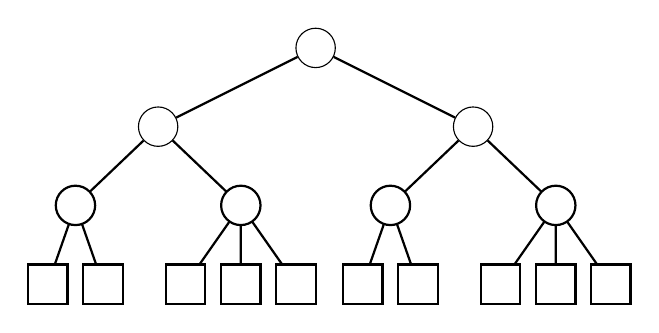
\begin{tikzpicture}[
	edge from parent/.style={draw, thick},
	every node/.style={draw, minimum size=5mm, inner sep=0pt},
	circ/.style={circle},
	sq/.style={rectangle},
	level distance=10mm,
	level 1/.style={sibling distance=40mm},
	level 2/.style={sibling distance=21mm},
	level 3/.style={sibling distance=7mm}
	]
	\node[circ] {}
	child { node[circ] {}
		child { node[circ] {}
			child { node[sq] {} }
			child { node[sq] {} }
		}
		child { node[circ] {}
			child { node[sq] {} }
			child { node[sq] {} }
			child { node[sq] {} }
		}
	}
	child { node[circ] {}
		child { node[circ] {}
			child { node[sq] {} }
			child { node[sq] {} }
		}
		child { node[circ] {}
			child { node[sq] {} }
			child { node[sq] {} }
			child { node[sq] {} }
		}
	};
\end{tikzpicture}
\end{lstlisting}
TikZ can draw trees using the pattern:
\[
\verb|\node {root} child { node {child1} } child { node {child2} };|
\]
\newpage
\begin{center}
	\includegraphics[scale=1]{tikzs/tree.pdf}
\end{center}

\paragraph{Key keywords}
\begin{itemize}
	\item \verb|\node ...;| creates the root node.
	\item \verb|child { ... }| creates a child subtree.
	\item Every \verb|child| contains another \verb|node|, which becomes the child node.
	\item Indentation is not required, but it helps you see the structure.
\end{itemize}

%----------------------------------------------------------
\subsubsection{Understanding the Style Block (The Part in [ ... ])}
%----------------------------------------------------------
At the top:\[
\verb|\begin{tikzpicture}[ ... ]|
\]
Everything inside \verb|[ ... ]| sets default styles and spacing.
\[
\verb|edge from parent/.style={draw, thick}|
\]
This means: every edge connecting a parent to a child is drawn as a thick line.
\[
\verb|every node/.style={draw, minimum size=5mm, inner sep=0pt}|
\]
This sets defaults for all nodes:
\begin{itemize}
	\item \verb|draw| draws the node border.
	\item \verb|minimum size=5mm| makes nodes at least 5mm in width/height.
	\item \verb|inner sep=0pt| removes extra padding inside nodes.
\end{itemize}
\[
\verb|circ/.style={circle}|
\qquad
\verb|sq/.style={rectangle}|
\]
These are \textbf{named styles} you can reuse:
\begin{itemize}
	\item \verb|node[circ]| makes a circular node.
	\item \verb|node[sq]| makes a rectangular node.
\end{itemize}
	
\newpage
%----------------------------------------------------------
\subsubsection{Spacing Control (Preventing Overlap)}
%----------------------------------------------------------
TikZ places nodes in levels (root at level 0, its children at level 1, etc.).
	
\[
\verb|level distance=10mm|
\]
This is the distance between one level and the next (vertical gap).
	
\[
\verb|level 1/.style={sibling distance=40mm}|
\]
\[
\verb|level 2/.style={sibling distance=21mm}|
\]
\[
\verb|level 3/.style={sibling distance=7mm}|
\]
\begin{itemize}
	\item \textbf{sibling distance} controls how far apart children of the same parent are.
	\item We give a larger distance near the top (level 1) because the big left and right subtrees
	must not overlap.
	\item Lower levels can use smaller distances because their subtrees are narrower.
\end{itemize}
	
%----------------------------------------------------------
\subsubsection{Reading the Tree Structure}
%----------------------------------------------------------
Start with the root:
\[
\verb|\node[circ] {}|
\]
This creates one circle (the root).
	
Then the root has \textbf{two children} because it has two \verb|child {...}| blocks:
\begin{itemize}
	\item First \verb|child {...}| is the left subtree.
	\item Second \verb|child {...}| is the right subtree.
\end{itemize}
	
\paragraph{Inside one subtree}
Example (left subtree):
\begin{lstlisting}
child { node[circ] {}
	child { node[circ] { ... } }
	child { node[circ] { ... } }
}
\end{lstlisting}
That means:
\begin{itemize}
	\item A circular node (level 1),
	\item with two circular children (level 2),
	\item each of which has several square leaves (level 3).
\end{itemize}

	
\newpage
\subsection{Building a One-Class SVM Figure with TikZ}
%----------------------------------------------------------
\paragraph{Learning Goals}
%----------------------------------------------------------
After this lesson, students should be able to:
\begin{itemize}
	\item Build a complex TikZ diagram using \textbf{structured blocks}.
	\item Use \verb|\def| parameters to control the picture (window size, origin position, slope, margin).
	\item Draw \textbf{axes} with an \textbf{off-center origin}.
	\item Plot lines defined by an equation (hyperplane and margins).
	\item Place points using \verb|\foreach| and basic coordinate arithmetic.
	\item Create annotated elements: arrows, labels, legend, and caption.
\end{itemize}
%The diagram is a common visualization for \textbf{one-class Support Vector Machines (SVM)}.
%It includes:
%\begin{itemize}
%	\item A feature space with axes $\Phi(x_1)$ and $\Phi(x_2)$.
%	\item A separating hyperplane (red solid line) and two margin boundaries (red dashed lines).
%	\item Training samples (black dots) representing the \emph{normal class}.
%	\item Support vectors (circled black dots) lying on/near the margin.
%	\item Samples violating the constraint (gray balls) labeled by slack variables $\xi_i,\xi_j$.
%	\item A legend explaining marker types.
%\end{itemize}

\begin{lstlisting}
\begin{tikzpicture}[scale=0.95, line cap=round, line join=round]
	
	% ----------------------------
	% 0) Canvas box
	% ----------------------------
	\def\xmin{-7} \def\xmax{7}
	\def\ymin{-7} \def\ymax{7}
	\draw[thick] (\xmin,\ymin-2) rectangle (\xmax,\ymax);
	
	% ----------------------------
	% 1) Off-center origin (like the figure)
	% ----------------------------
	\def\Ox{-2.4}
	\def\Oy{-1.2}
	\coordinate (O) at (\Ox,\Oy);
	
	\begin{scope}
		\clip (\xmin,\ymin) rectangle (\xmax,\ymax);
		
		% ----------------------------
		% 2) Axes
		% ----------------------------
		\draw[blue!70, very thick, ->] (\xmin+0.5,\Oy) -- (\xmax-1.5,\Oy)
		node[right] {$\Phi(x_1)$};
		\draw[blue!70, very thick, ->] (\Ox,\ymin+0.5) -- (\Ox,\ymax-1)
		node[above] {$\Phi(x_2)$};
		
		\fill[blue!80] (O) circle (4pt);
		\node[below left] at (O) {Origin};
		
		% ----------------------------
		% 3) Hyperplane + two margins (parallel)
		%    y - Oy = m(x - Ox) + c
		% ----------------------------
		\def\m{-1.05}   % slope
		\def\c{2.0}     % shift
		\def\dm{2}      % margin spacing
		
		% solid hyperplane
		\draw[red, very thick]
		(\xmin,{ \Oy + \m*(\xmin-\Ox) + \c }) --
		(\xmax,{ \Oy + \m*(\xmax-\Ox) + \c })
		node[pos=0.75, rotate=-46, black, above] {Optimal hyperplane};
		
		% dashed margins
		\draw[red, dashed, thick]
		(\xmin,{ \Oy + \m*(\xmin-\Ox) + \c + \dm }) --
		(\xmax,{ \Oy + \m*(\xmax-\Ox) + \c + \dm });
		
		\draw[red, dashed, thick]
		(\xmin,{ \Oy + \m*(\xmin-\Ox) + \c - \dm }) --
		(\xmax,{ \Oy + \m*(\xmax-\Ox) + \c - \dm });
		
		\node[rotate=-46] at (\Ox-3.5,\Oy+6.0) {$\textbf{w}\cdot \textbf{x} + b = 0$};
		
		% ----------------------------
		% 4) Margin arrow
		% ----------------------------
		\draw[gray, very thick, <->] (\Ox-1,\Oy+5) -- (\Ox-2.9,\Oy+3.1)
		node[gray!50!black, sloped, above, midway, font=\bfseries] {Margin};
		
		% ----------------------------
		% 5) w arrow
		% ----------------------------
		\draw[blue!70, very thick, ->] (\Ox+.5,\Oy+1.5) -- (\Ox+1,\Oy+2)
		node[sloped, above, midway] {$\textbf{w}$};
		
		% ----------------------------
		% 6) Normal class points (black cluster)
		% ----------------------------
		\foreach \p in {
			(0.9,4.1),(0.1,3.3),(1.7,3.4),(1.2,2.7),(0.4,2.6),
			(2.2,2.5),(0.5,1.9),(1.6,1.7),(2.5,1.7),(1.1,1.2),
			(2.1,1.1),(0.6,0.9),(1.5,0.5),(2.3,0.5),
			(1.2,1.9),(1.9,2.0)
		}{
			\fill \p circle (4pt);
		}
		
		% ----------------------------
		% 7) Support vectors (circled points)
		% ----------------------------
		\foreach \p in {(\Ox+2,\Oy+1.9), (\Ox+1,\Oy+2.9), (\Ox+3,\Oy+.9)}{
			\fill \p circle (4pt);
			\draw \p circle (7pt);
		}
		
		% ----------------------------
		% 8) Samples violating constraint (gray balls) + xi labels
		% ----------------------------
		\shade[ball color=gray!60] (\Ox+1,\Oy+.25) circle (5pt) node[above=2pt] {$\xi_i$};
		\shade[ball color=gray!60] (\Ox+1.75,\Oy-.5) circle (5pt) node[below=2pt] {$\xi_j$};
	\end{scope}
	
	% ----------------------------
	% 9) Legend box
	% ----------------------------
	\begin{scope}[shift={(0,-8)}]
		\draw[blue!60, fill=white, thick, rounded corners=4pt] (-4.5,-.75) rectangle (4.5,1.0);
		
		\fill (-4,0.5) circle (5pt) node[right=4pt] {Normal class};
		\draw (-.5,.5) circle (5pt) node[right=4pt] {Support vector};
		\shade[ball color=gray!60] (-.5,-0.25) circle (5pt) node[right=4pt] {Sample violating constraint};
	\end{scope}
	
	% ----------------------------
	% 10) Caption (optional)
	% ----------------------------
	\node at (0,-9.5) {Fig.\ 2.\quad One-class Support Vector Machine};
	
\end{tikzpicture}
\end{lstlisting}
\begin{center}
	\includegraphics[scale=.9]{tikzs/OCSVM.pdf}
\end{center}


\subsubsection{Block 0: Canvas box (plot window)}
\begin{itemize}
	\item The macros \verb|\xmin,\xmax,\ymin,\ymax| define the drawing window.
	\item The rectangle frames the figure:
\end{itemize}
\[
\verb|\draw[thick] (\xmin,\ymin-2) rectangle (\xmax,\ymax);|
\]
\textbf{Teaching tip:} Ask students why \verb|\ymin-2| is used (to make extra room for the legend/caption).

\subsubsection{Block 1: Off-center origin}
\[
\verb|\def\Ox{-2.4} \def\Oy{-1.2}|
\]
\[
\verb|\coordinate (O) at (\Ox,\Oy);|
\]
This is the most important design choice: the axes cross at (\verb*|\Ox|,\verb*|\Oy|) rather than $(0,0)$, matching the reference figure.

\subsubsection{Why we use \texttt{scope} + \texttt{clip}}
\[
\verb|\begin{scope} ... \clip ... \end{scope}|
\]
Everything inside this scope is clipped to the rectangle:
\begin{itemize}
	\item prevents lines and points from spilling outside,
	\item keeps the final graphic clean.
\end{itemize}

\subsubsection{Block 2: Axes with arrowheads and labels}
Key idea: use $(\verb*|\xmin|,\verb*|\Oy|)$ and $(\verb*|\Ox|,\verb*|\ymin|)$ to align axes with the off-center origin.

\[
\verb|(\xmin+0.5,\Oy) -- (\xmax-1.5,\Oy)|
\]
creates the horizontal axis across $y=\verb*|\Oy|$.

\[
\verb|(\Ox,\ymin+0.5) -- (\Ox,\ymax-1)|
\]
creates the vertical axis across $x=\verb*|\Ox|$.

\subsubsection{Block 3: Hyperplane and margins (equation-driven drawing)}
The hyperplane is defined by the shifted line equation:
\[
y - \verb*|\Oy| = m(x - \verb*|\Ox|) + c.
\]
So if we pick a value of $x$, TikZ computes $y$ by:
\[
y = \verb*|\Oy| + m(x-\verb*|\Ox|) + c.
\]
This is why the endpoints are written like:
\[
\verb|(\xmin,{ \Oy + \m*(\xmin-\Ox) + \c })|
\]

\paragraph{Margins.}
The dashed margins are parallel lines obtained by shifting $c$:
\[
c \to c+\mathrm{dm}\quad\text{and}\quad c\to c-\mathrm{dm}.
\]
In code, that is:
\[
\verb|... + \dm| \quad \text{and} \quad \verb|... - \dm|
\]

\subsubsection{Block 4: Margin arrow}
\[
\verb|\draw[gray, very thick, <->] (A) -- (B) node[...] {Margin};|
\]
\begin{itemize}
	\item \verb|<->| puts arrowheads on both ends.
	\item \verb|sloped| rotates the label to match the arrow direction.
	\item \verb|midway| puts the label in the middle.
\end{itemize}

\subsubsection{Block 5: The $\mathbf{w}$ direction arrow}
This arrow is a visual cue for the normal vector direction.
\[
\verb|(\Ox+.5,\Oy+1.5) -- (\Ox+1,\Oy+2)|
\]
Notice: these coordinates are written relative to $(\verb*|\Ox|,\verb*|\Oy|)$ so they move naturally if the origin moves.

\subsubsection{Block 6: Plotting the normal class points}
The code uses:
\[
\verb|\foreach \p in { (x1,y1),(x2,y2),... }{ \fill \p circle (4pt); }|
\]
This is the easiest way to plot many points:
\begin{itemize}
	\item Put point coordinates in the list.
	\item TikZ loops through them and plots each dot.
\end{itemize}

\subsubsection{Block 7: Support vectors (circled points)}
Support vectors are shown as a dot plus a surrounding circle:
\[
\verb|\fill \p circle (4pt);|
\quad \text{and} \quad
\verb|\draw \p circle (7pt);|
\]

\subsubsection{Block 8: Violating samples with shading}
The command:
\[
\verb|\shade[ball color=gray!60] (x,y) circle (5pt);|
\]
creates a nice “3D ball” effect. Then a node attaches the label $\xi_i$ or $\xi_j$.

\subsubsection{Block 9: Legend box}
The legend is drawn in a shifted scope:
\[
\verb|\begin{scope}[shift={(0,-8)}] ... \end{scope}|
\]
This moves the legend down without rewriting every coordinate.

Inside the legend, three marker types are drawn using:
\begin{itemize}
	\item \verb|\fill ... circle| for normal class,
	\item \verb|\draw ... circle| for support vectors (outline only),
	\item \verb|\shade ... circle| for violating samples.
\end{itemize}

%\subsubsection{Block 10: Caption}
%A simple \verb|\node| places the caption at a fixed coordinate.

%%----------------------------------------------------------
%\subsubsection{Parameters Students Can Experiment With}
%%----------------------------------------------------------
%Encourage students to change these and recompile:
%\begin{itemize}
%	\item \verb|\Ox,\Oy|: move the origin and see everything reposition correctly.
%	\item \verb|\m|: rotate the hyperplane (change slope).
%	\item \verb|\c|: shift the hyperplane up/down relative to the origin.
%	\item \verb|\dm|: widen/narrow the margin.
%	\item point coordinates: reshape the class distribution.
%\end{itemize}


%\chapter{Introduction to \LaTeX}

\section{What is \LaTeX?}

\LaTeX{} (pronounced either “Lay-tek” or “Lah-tek”) is a high-quality typesetting system designed for producing scientific and technical documents. It separates content from formatting, allowing authors to focus on writing rather than visual layout.

\begin{definition}[LaTeX]
	\LaTeX{} is a document preparation system based on \TeX{}, designed for the creation of beautifully typeset documents, especially those containing complex mathematical expressions.
\end{definition}

\subsection{Why Use \LaTeX?}

Some benefits of using \LaTeX{} include:

\begin{itemize}
	\item Professional-quality typesetting
	\item Excellent mathematical rendering (e.g., $a^2 + b^2 = c^2$)
	\item Automated references, bibliographies, and table of contents
	\item Consistent document structure and style
\end{itemize}

\section{Compiling a Document}

To convert a `.tex` file into a PDF, you need to compile it using a LaTeX engine such as `pdflatex`.

\begin{verbatim}
	pdflatex file.tex
	pdflatex file.tex  % Run twice for updated references
\end{verbatim}

\subsection{Recommended Tools}

\begin{itemize}
	\item \textbf{Overleaf}: Online editor, no installation required.
	\item \textbf{TeX Live}: Comprehensive distribution for Linux/macOS.
	\item \textbf{MiKTeX}: User-friendly distribution for Windows.
\end{itemize}

\section{Minimal Example}

Every LaTeX document consists of two main parts:

\begin{itemize}
	\item \textbf{Preamble} (before \verb|\begin{document}|): specifies the document class and packages
		\item \textbf{Body} (between \verb|\begin{document}| and \verb|\end{document}|): contains the actual content
	\end{itemize}
	
	\begin{example}[Minimal Document]
		\begin{verbatim}
			\documentclass{article}
			
			\begin{document}
				Hello, world! $E = mc^2$
			\end{document}
		\end{verbatim}
	\end{example}
	
	\section{Chapter Summary}
	
	\begin{itemize}
		\item LaTeX is a powerful typesetting system.
		\item Compilation turns source code into a PDF.
		\item Use \verb|pdflatex| or Overleaf to build your documents.
	\end{itemize}
	
	\begin{exercise}
		Install Overleaf or a local TeX distribution. Create a `.tex` file with a simple "Hello, world!" message and compile it.
	\end{exercise}

%\chapter{Document Structure and Classes}

\section{Anatomy of a LaTeX Document}

A LaTeX file is a plain text file with the `.tex` extension. It typically has two main parts:

\begin{itemize}
	\item The \textbf{preamble}, where you set document options and load packages.
	\item The \textbf{document body}, where you write content.
\end{itemize}

\begin{example}[Minimal Structure]
	\begin{verbatim}
		\documentclass{article}
		
		\begin{document}
			This is a LaTeX document.
		\end{document}
	\end{verbatim}
\end{example}

\section{Document Classes}

The \verb|\documentclass| command defines the type of document.

\begin{itemize}
	\item \texttt{article} – for short papers, homework, notes
	\item \texttt{report} – for longer documents with chapters
	\item \texttt{book} – for writing books with two-sided layout
	\item \texttt{beamer} – for presentations
\end{itemize}

\begin{example}
	\verb|\documentclass[12pt]{report}|
\end{example}

\section{Class Options}

You can add options to customize your document:

\begin{itemize}
	\item \texttt{10pt}, \texttt{11pt}, \texttt{12pt} — font size
	\item \texttt{a4paper}, \texttt{letterpaper} — paper size
	\item \texttt{twoside}, \texttt{oneside} — page layout
	\item \texttt{twocolumn} — two-column text
\end{itemize}

\begin{example}
	\verb|\documentclass[12pt, a4paper, twoside]{article}|
\end{example}

\section{Packages}

Packages extend LaTeX’s capabilities. Load them in the preamble:

\begin{verbatim}
	\usepackage{amsmath, amssymb}
	\usepackage{graphicx}
	\usepackage{hyperref}
\end{verbatim}

\begin{definition}[Package]
	A LaTeX package is a collection of macros and commands that add functionality. Use \verb|\usepackage{...}| to load it.
\end{definition}

\section{Skeleton Template}

\begin{example}[Typical Structure]
	\begin{verbatim}
		\documentclass[11pt]{article}
		\usepackage[utf8]{inputenc}
		\usepackage{amsmath, amssymb}
		\usepackage{graphicx}
		\usepackage{hyperref}
		
		\title{My First Document}
		\author{Student Name}
		\date{\today}
		
		\begin{document}
			\maketitle
			
			Hello, LaTeX World!
			
		\end{document}
	\end{verbatim}
\end{example}

\section{Exercise}

\begin{exercise}
	Create a new LaTeX file with:
	\begin{itemize}
		\item Class: \texttt{report}
		\item Title: “My LaTeX Project”
		\item Use packages: \texttt{amsmath}, \texttt{graphicx}, \texttt{hyperref}
		\item Display a simple sentence: “This is my LaTeX report.”
	\end{itemize}
\end{exercise}

%\chapter{Text Formatting and Layout}

\section{Basic Text Commands}

LaTeX provides a variety of text formatting commands to style your writing.

\begin{itemize}
	\item \verb|\textbf{bold}| → \textbf{bold}
	\item \verb|\textit{italic}| → \textit{italic}
	\item \verb|\underline{underline}| → \underline{underline}
	\item \verb|\emph{emphasized}| → \emph{emphasized} (contextual)
\end{itemize}

\begin{example}
	This is \textbf{bold}, \textit{italic}, and \underline{underlined}.
\end{example}

\section{Paragraphs and Line Breaks}

\begin{itemize}
	\item A blank line starts a new paragraph.
	\item Use \verb|\\| for a manual line break.
\end{itemize}

\begin{example}
	This is the first line.\\
	This is the second line.
\end{example}

\section{Quotes and Verbatim Text}

\begin{itemize}
	\item Use \verb|\verb| for short inline code: \verb|\LaTeX|.
	\item Use the \texttt{verbatim} environment for code blocks.
	\item Use \texttt{quote} or \texttt{quotation} for indented blocks.
\end{itemize}

\begin{example}
	\begin{verbatim}
		\begin{itemize}
			\item First
			\item Second
		\end{itemize}
	\end{verbatim}
\end{example}

\section{Text Alignment}

\begin{itemize}
	\item \verb|\begin{center}...\end{center}| → centered text
	\item \verb|\begin{flushleft}...\end{flushleft}| → left-aligned
	\item \verb|\begin{flushright}...\end{flushright}| → right-aligned
\end{itemize}

\begin{example}
	\begin{center}
		This is centered.
	\end{center}
\end{example}

\section{Font Sizes}

\LaTeX{} supports relative font sizes:

\begin{itemize}
	\item \verb|\tiny|, \verb|\scriptsize|, \verb|\footnotesize|
	\item \verb|\small|, \verb|\normalsize|, \verb|\large|, \verb|\Large|
	\item \verb|\LARGE|, \verb|\huge|, \verb|\Huge|
\end{itemize}

\begin{example}
	{\Large This is large text.}
\end{example}

\section{Special Characters}

Some characters must be escaped using a backslash:

\begin{tabular}{ll}
	\verb|\%| & \% (percent) \\
	\verb|\$| & \$ (dollar) \\
	\verb|\#| & \# (hash) \\
	\verb|\_| & \_ (underscore) \\
	\verb|\&| & \& (ampersand) \\
	\verb|\{| \verb|\}| & \{ \}, braces
\end{tabular}

\section{Comments}

Use the percent symbol (\verb|%|) to add comments:

\begin{verbatim}
	% This is a comment and will not appear in the output
\end{verbatim}

\section{Exercise}

\begin{exercise}
	Create a document with:
	\begin{itemize}
		\item A centered title using \verb|\begin{center}|
			\item A paragraph using \verb|\textit| and \verb|\textbf|
			\item One inline verbatim command using \verb|\verb|
			\item A list of three escaped special characters
		\end{itemize}
	\end{exercise}

%\chapter{Lists, Tables, and Environments}

\section{Unordered Lists (Bulleted)}

Use the \texttt{itemize} environment to create bulleted lists.

\begin{example}
	\begin{verbatim}
		\begin{itemize}
			\item Apples
			\item Bananas
			\item Cherries
		\end{itemize}
	\end{verbatim}
\end{example}

\begin{itemize}
	\item Apples
	\item Bananas
	\item Cherries
\end{itemize}

\section{Ordered Lists (Numbered)}

Use the \texttt{enumerate} environment for numbered lists.

\begin{example}
	\begin{verbatim}
		\begin{enumerate}
			\item First
			\item Second
			\item Third
		\end{enumerate}
	\end{verbatim}
\end{example}

\begin{enumerate}
	\item First
	\item Second
	\item Third
\end{enumerate}

\section{Description Lists}

Use the \texttt{description} environment for labeled items.

\begin{example}
	\begin{verbatim}
		\begin{description}
			\item[Dog] A friendly animal.
			\item[Cat] A curious animal.
		\end{description}
	\end{verbatim}
\end{example}

\begin{description}
	\item[Dog] A friendly animal.
	\item[Cat] A curious animal.
\end{description}

\section{Tables with \texttt{tabular}}

Use the \texttt{tabular} environment to create tables.

\begin{example}
	\begin{verbatim}
		\begin{tabular}{|l|c|r|}
			\hline
			Name & Age & Score \\
			\hline
			Alice & 24 & 95 \\
			Bob & 22 & 88 \\
			\hline
		\end{tabular}
	\end{verbatim}
\end{example}

\begin{center}
	\begin{tabular}{|l|c|r|}
		\hline
		Name & Age & Score \\
		\hline
		Alice & 24 & 95 \\
		Bob & 22 & 88 \\
		\hline
	\end{tabular}
\end{center}

\section{Alignment Options in Tables}

\begin{itemize}
	\item \texttt{l} – left aligned
	\item \texttt{c} – centered
	\item \texttt{r} – right aligned
	\item \texttt{|} – vertical line between columns
\end{itemize}

\section{Floating Tables}

For floating tables with captions and labels, use the \texttt{table} environment:

\begin{example}
	\begin{verbatim}
		\begin{table}[h]
			\centering
			\begin{tabular}{lrr}
				\hline
				Item & Qty & Price \\
				\hline
				Apples & 3 & 1.20 \\
				Bananas & 5 & 0.80 \\
				\hline
			\end{tabular}
			\caption{Fruit Inventory}
			\label{tab:fruit}
		\end{table}
	\end{verbatim}
\end{example}

\section{Custom Environments}

LaTeX also supports custom environments like \texttt{quote}, \texttt{verbatim}, and math environments (coming soon in Chapter 5).

\begin{example}
	\begin{quote}
		"LaTeX is worth learning." -- Every LaTeX user
	\end{quote}
\end{example}

\section{Exercise}

\begin{exercise}
	Create a document with:
	\begin{itemize}
		\item An unordered list of 3 programming languages
		\item A table listing 3 students and their scores
		\item A floating table with a caption and label
		\item A short quote in the \texttt{quote} environment
	\end{itemize}
\end{exercise}

%\chapter{Mathematical Typesetting}

\section{Why LaTeX is Powerful for Mathematics}

One of the strongest reasons to use LaTeX is its ability to typeset mathematics clearly and professionally. Mathematical notation in LaTeX is precise, readable, and consistent across documents.

\section{Inline and Display Mathematics}

\subsection{Inline Mathematics}

Inline mathematics is used inside a sentence and must be enclosed in dollar signs.  
For example, the famous equation $E = mc^2$ appears naturally within text.

\begin{example}
	The quadratic polynomial $ax^2 + bx + c$ has degree $2$.
\end{example}

\subsection{Displayed Mathematics}

Displayed mathematics is used for important equations that appear on their own line.

\begin{equation}
	E = mc^2
\end{equation}

\section{Superscripts and Subscripts}

\begin{itemize}
	\item Superscripts use the caret symbol: $x^2$, $a^{n+1}$
	\item Subscripts use the underscore symbol: $a_1$, $b_{ij}$
\end{itemize}

\begin{example}
	The sequence $a_n = n^2$ grows quadratically.
\end{example}

\section{Fractions and Roots}

\begin{itemize}
	\item Fractions: $\frac{a}{b}$
	\item Nested fractions: $\frac{1}{1 + \frac{1}{x}}$
	\item Square roots: $\sqrt{2}$
	\item General roots: $\sqrt[n]{x}$
\end{itemize}

\begin{example}
	The solution is $x = \frac{-b \pm \sqrt{b^2 - 4ac}}{2a}$.
\end{example}

\section{Greek Letters}

Greek letters are frequently used in mathematics and science.

\begin{itemize}
	\item Lowercase: $\alpha$, $\beta$, $\gamma$, $\delta$, $\epsilon$
	\item Uppercase: $\Gamma$, $\Delta$, $\Theta$, $\Lambda$
\end{itemize}

\section{Common Mathematical Symbols}

\begin{itemize}
	\item Summation: $\sum_{i=1}^{n} i$
	\item Product: $\prod_{k=1}^{n} k$
	\item Integrals: $\int_0^1 x^2 \, dx$
	\item Limits: $\lim_{x \to 0} \frac{\sin x}{x}$
\end{itemize}

\section{Aligned Equations}

Use the \texttt{align} environment to align multiple equations.

\begin{align}
	x + y &= 10 \\
	2x - y &= 3
\end{align}

\section{Matrices}

Matrices are written using matrix environments.

\begin{equation}
	A =
	\begin{pmatrix}
		1 & 2 \\
		3 & 4
	\end{pmatrix}
\end{equation}

\section{Cases}

Piecewise-defined functions use the \texttt{cases} environment.

\begin{equation}
	f(x) =
	\begin{cases}
		x^2, & x \geq 0 \\
		-x, & x < 0
	\end{cases}
\end{equation}

\section{Exercise}

\begin{exercise}
	Typeset the following in LaTeX:
	\begin{itemize}
		\item The binomial formula $(a+b)^2 = a^2 + 2ab + b^2$
		\item A $2 \times 3$ matrix
		\item The definite integral $\int_0^\pi \sin x \, dx$
		\item A piecewise function with two cases
	\end{itemize}
\end{exercise}

%\chapter{Theorems, Definitions, and Proofs}

\section{Using the \texttt{amsthm} Package}

To define theorem-style environments in LaTeX, we use the \texttt{amsthm} package.

In your preamble, define environments like so:

\begin{verbatim}
	\usepackage{amsthm}
	
	\newtheorem{theorem}{Theorem}[chapter]
	\newtheorem{lemma}[theorem]{Lemma}
	\newtheorem{definition}[theorem]{Definition}
	\newtheorem{corollary}[theorem]{Corollary}
	\theoremstyle{remark}
	\newtheorem*{remark}{Remark}
\end{verbatim}

\section{Basic Environments}

\begin{definition}[Even Number]
	An integer $n$ is called \emph{even} if there exists an integer $k$ such that $n = 2k$.
\end{definition}

\begin{theorem}[Sum of Evens]
	The sum of two even integers is even.
\end{theorem}

\begin{proof}
	Let $a = 2m$ and $b = 2n$ for some integers $m$ and $n$.  
	Then $a + b = 2m + 2n = 2(m + n)$, which is divisible by $2$.  
	Therefore, $a + b$ is even.
\end{proof}

\section{More Structures}

\begin{lemma}[Basic Algebra]
	If $a^2 = b^2$, then $a = b$ or $a = -b$.
\end{lemma}

\begin{corollary}
	If $x^2 = 9$, then $x = 3$ or $x = -3$.
\end{corollary}

\begin{remark}
	You can group lemmas, theorems, and corollaries using the same counter by specifying it in square brackets.
\end{remark}

\section{Proof Formatting Tips}

\begin{itemize}
	\item Use short paragraphs inside proofs.
	\item Always close proofs with \verb|\qed| or let LaTeX do it automatically.
	\item Avoid long inline equations in proofs; prefer display mode if clarity is needed.
\end{itemize}

\section{Example: The Pythagorean Theorem}

\begin{theorem}[Pythagorean Theorem]
	In a right triangle with legs $a$, $b$ and hypotenuse $c$, we have:
	\[
	c^2 = a^2 + b^2
	\]
\end{theorem}

\begin{proof}
	There are many geometric and algebraic proofs. One method involves comparing the area of squares built on each side.
\end{proof}

\section{Exercise}

\begin{exercise}
	Define your own:
	\begin{itemize}
		\item A definition for a "prime number"
		\item A theorem stating: “If $p$ is prime and $p$ divides $ab$, then $p$ divides $a$ or $p$ divides $b$.”
		\item A brief proof using basic divisibility
	\end{itemize}
\end{exercise}

%\chapter{Figures and Graphics}

\section{Including Images with \texttt{graphicx}}

To insert images in LaTeX, use the \texttt{graphicx} package:

\begin{verbatim}
	\usepackage{graphicx}
\end{verbatim}

\section{Basic Usage: \texttt{\textbackslash includegraphics}}

Use the \verb|\includegraphics| command inside a \texttt{figure} environment to insert images with captions and labels.

\begin{example}[Simple Figure]
	\begin{verbatim}
		\begin{figure}[h]
			\centering
			\includegraphics[width=0.6\textwidth]{example-image}
			\caption{An example image}
			\label{fig:example}
		\end{figure}
	\end{verbatim}
\end{example}

\begin{remark}
	To compile images successfully:
	\begin{itemize}
		\item Use `.png`, `.jpg`, or `.pdf` formats (depending on engine).
		\item Ensure image files are in the same folder as your `.tex` file.
	\end{itemize}
\end{remark}

\section{Controlling Image Size}

You can adjust the size using:

\begin{itemize}
	\item \verb|width=...| e.g., \verb|width=0.5\textwidth|
	\item \verb|height=...| e.g., \verb|height=4cm|
	\item \verb|scale=...| e.g., \verb|scale=0.8|
\end{itemize}

\begin{example}
	\verb|\includegraphics[scale=0.5]{diagram}|
\end{example}

\section{Positioning Figures}

You can use optional arguments for placement:

\begin{itemize}
	\item \texttt{h} — here
	\item \texttt{t} — top of page
	\item \texttt{b} — bottom of page
	\item \texttt{p} — on a separate page of floats
\end{itemize}

Example: \verb|\begin{figure}[htbp]|
	
	\section{Referencing Figures}
	
	Use \verb|\label| and \verb|\ref| to refer to figures.
	
	\begin{example}
		See Figure~\ref{fig:example} for a visual illustration.
	\end{example}
	
	\section{Side-by-Side Images}
	
	Use the \texttt{minipage} environment to place multiple images side by side:
	
	\begin{example}
		\begin{verbatim}
			\begin{figure}[h]
				\centering
				\begin{minipage}{0.45\textwidth}
					\centering
					\includegraphics[width=\textwidth]{img1}
					\caption{Image 1}
				\end{minipage}
				\hfill
				\begin{minipage}{0.45\textwidth}
					\centering
					\includegraphics[width=\textwidth]{img2}
					\caption{Image 2}
				\end{minipage}
			\end{figure}
		\end{verbatim}
	\end{example}
	
	\section{Exercise}
	
	\begin{exercise}
		Create a LaTeX document that:
		\begin{itemize}
			\item Loads the \texttt{graphicx} package
			\item Inserts an image of your choice with caption and label
			\item Places two images side by side
			\item Refers to the image using \verb|\ref|
		\end{itemize}
	\end{exercise}

%\chapter{Cross-Referencing and Labels}

\section{Why Use Cross-References?}

Cross-referencing allows you to:
\begin{itemize}
	\item Refer to sections, figures, tables, and equations dynamically
	\item Automatically update numbers when structure changes
	\item Improve document navigability, especially in long documents
\end{itemize}

\section{Basic Labeling Syntax}

Use \verb|\label{key}| to mark a location, and use \verb|\ref{key}| to refer to it later.

\begin{example}
	\begin{verbatim}
		\section{Methodology}
		\label{sec:method}
		
		As discussed in Section~\ref{sec:method}, we use...
	\end{verbatim}
\end{example}

\section{Referencing Figures and Tables}

\begin{itemize}
	\item Place \verb|\label| after \verb|\caption|
	\item Reference with \verb|\ref|
\end{itemize}

\begin{example}
	\begin{verbatim}
		\begin{figure}[h]
			\centering
			\includegraphics[width=0.5\textwidth]{plot}
			\caption{Data trend}
			\label{fig:trend}
		\end{figure}
		
		See Figure~\ref{fig:trend}.
	\end{verbatim}
\end{example}

\section{Referencing Equations}

For numbered equations:

\begin{verbatim}
	\begin{equation}
		a^2 + b^2 = c^2
		\label{eq:pythagoras}
	\end{equation}
	
	From Eq.~\eqref{eq:pythagoras}, we know...
\end{verbatim}

\section{Referencing Theorems and Definitions}

\begin{example}
	\begin{verbatim}
		\begin{theorem}
			\label{thm:addition}
			Addition of even numbers is even.
		\end{theorem}
		
		Theorem~\ref{thm:addition} proves the statement.
	\end{verbatim}
\end{example}

\section{Hyperlinks with \texttt{hyperref}}

To make all references clickable in the PDF, use the \texttt{hyperref} package:

\begin{verbatim}
	\usepackage{hyperref}
\end{verbatim}

\begin{itemize}
	\item \verb|\href{URL}{text}| — insert a clickable external link
	\item \verb|\url{URL}| — insert a plain clickable URL
\end{itemize}

\begin{example}
	\href{https://www.latex-project.org}{Visit the LaTeX Project}
\end{example}

\section{Best Practices}

\begin{itemize}
	\item Prefix label names: \texttt{sec:}, \texttt{fig:}, \texttt{eq:}, \texttt{thm:}, etc.
	\item Always run \LaTeX{} twice to update references.
\end{itemize}

\section{Exercise}

\begin{exercise}
	Write a LaTeX document that includes:
	\begin{itemize}
		\item A labeled section titled “Results”
		\item A numbered and labeled equation
		\item A figure with caption and label
		\item A clickable link to an external website
		\item Proper references using \verb|\ref| and \verb|\eqref|
	\end{itemize}
\end{exercise}

%\chapter{Bibliography and Citations}

\section{Why Cite?}

Citing sources:
\begin{itemize}
	\item Gives credit to original authors
	\item Supports your arguments with reliable references
	\item Helps readers find more information
\end{itemize}

\section{Manual Bibliography with \texttt{thebibliography}}

This is the simplest method and requires no external files.

\begin{example}
	\begin{verbatim}
		\begin{thebibliography}{9}
			
			\bibitem{knuth}
			D. E. Knuth,
			\textit{The \TeX{}book},
			Addison-Wesley, 1984.
			
			\bibitem{lamport}
			L. Lamport,
			\textit{\LaTeX: A Document Preparation System},
			2nd ed., Addison-Wesley, 1994.
			
		\end{thebibliography}
	\end{verbatim}
\end{example}

To cite a reference:

\begin{verbatim}
	As shown in \cite{knuth}, the TeX system is powerful.
\end{verbatim}

\section{Using BibTeX (Recommended for Larger Projects)}

With BibTeX, citations are stored in a separate `.bib` file.

\subsection*{Step 1: Create a File \texttt{references.bib}}

```bibtex
@book{knuth,
	author    = {Donald E. Knuth},
	title     = {The TeXbook},
	year      = {1984},
	publisher = {Addison-Wesley}
}

@article{einstein,
	author  = {Albert Einstein},
	title   = {Does the Inertia of a Body Depend Upon Its Energy Content?},
	journal = {Annalen der Physik},
	year    = {1905}
}
```


\subsection*{Step 2: In Your LaTeX Document}

\begin{verbatim}
	\bibliographystyle{plain}
	\bibliography{references}
\end{verbatim}

Cite references in the document using:

\begin{verbatim}
	Einstein explained this in \cite{einstein}.
\end{verbatim}

\section{Modern Approach: \texttt{biblatex} + \texttt{biber}}

More flexible and recommended for modern documents.

\begin{verbatim}
	\usepackage[backend=biber, style=alphabetic]{biblatex}
	\addbibresource{references.bib}
\end{verbatim}

Then compile using \texttt{pdflatex → biber → pdflatex → pdflatex}.

\subsection*{Cite Commands}

\begin{itemize}
	\item \verb|\cite{key}| – basic citation
	\item \verb|\parencite{key}| – citation in parentheses
	\item \verb|\textcite{key}| – citation as part of the sentence
\end{itemize}

\section{Citation Styles}

Change the style with the style= option:
\begin{itemize}
	\item numeric — [1], [2]
	\item alphabetic — [Knu84]
	\item authoryear — (Knuth, 1984)
	\item apa — APA style
\end{itemize}

\section{Exercise}

\begin{exercise}
	Create a document that:
	\begin{itemize}
		\item Uses either \texttt{thebibliography} or \texttt{biblatex}
		\item Adds at least two references (book + article)
		\item Cites both references in the document body
		\item Uses a citation style other than the default
	\end{itemize}
\end{exercise}
%\chapter{Custom Commands and Macros}

\section{Why Define Custom Commands?}

Custom commands:
\begin{itemize}
	\item Reduce repetition
	\item Make documents easier to maintain
	\item Clarify meaning through notation
\end{itemize}

\section{Defining New Commands}

Use the \verb|\newcommand| macro in the preamble to define your own commands.

\subsection*{Syntax}

\begin{verbatim}
	\newcommand{\name}{replacement text}
	\newcommand{\name}[n]{replacement with #1 to #n}
\end{verbatim}

\subsection*{Examples}

\begin{verbatim}
	\newcommand{\R}{\mathbb{R}}      % Real numbers
	\newcommand{\vect}[1]{\mathbf{#1}}  % Bold vectors
	\newcommand{\abs}[1]{\left|#1\right|}  % Absolute value
\end{verbatim}

\subsection*{Usage}

%\begin{itemize}
%	\item $\R$ denotes the set of real numbers
%	\item $\vect{v}$ is a vector
%	\item $\abs{x}$ gives the absolute value of $x$
%\end{itemize}

\section{Optional Arguments}

You can define optional arguments using \verb|\newcommand| with defaults:

\begin{verbatim}
	\newcommand{\set}[2][n]{\{#2_1, #2_2, \dots, #2_#1\}}
\end{verbatim}

\begin{itemize}
	\item \verb|\set{a}| produces $\{a_1, a_2, \dots, a_n\}$
	\item \verb|\set[3]{x}| produces $\{x_1, x_2, x_3\}$
\end{itemize}

\section{Renewing Existing Commands}

To override an existing command (use with caution):

\begin{verbatim}
	\renewcommand{\phi}{\varphi}
\end{verbatim}

\section{Declaring Math Operators}

For defining math-style functions:

\begin{verbatim}
	\DeclareMathOperator{\Var}{Var}
	\DeclareMathOperator*{\argmax}{arg\,max}
\end{verbatim}

Usage:
%\[
%\Var(X) \qquad \argmax_{x \in A} f(x)
%\]

\section{Best Practices}

\begin{itemize}
	\item Prefix your custom commands to avoid naming conflicts.
	\item Use clear, descriptive names (e.g., \verb|\vect| instead of \verb|\v|).
	\item Avoid redefining built-in commands unless absolutely necessary.
\end{itemize}

\section{Exercise}

\begin{exercise}
	In a LaTeX document:
	\begin{itemize}
		\item Define the following custom commands:
		\begin{itemize}
			\item \verb|\Z| for $\mathbb{Z}$
			\item \verb|\norm{x}| for $\left\|x\right\|$
			\item \verb|\inner{u}{v}| for inner product $\langle u, v \rangle$
		\end{itemize}
		\item Use each command in a math environment.
	\end{itemize}
\end{exercise}

%\chapter{Presentations with Beamer}

\section{What is Beamer?}

\texttt{beamer} is a LaTeX document class for creating high-quality presentations. It uses frames (slides) instead of pages and provides built-in themes, templates, and transitions.

\section{Basic Beamer Document}

\begin{verbatim}
	\documentclass{beamer}
	\usetheme{Madrid}
	
	\title{My First Beamer Presentation}
	\author{Your Name}
	\date{\today}
	
	\begin{document}
		
		\frame{\titlepage}
		
		\begin{frame}{Outline}
			\tableofcontents
		\end{frame}
		
		\section{Introduction}
		
		\begin{frame}{Why Beamer?}
			\begin{itemize}
				\item Professional slides
				\item Integrated with math and references
				\item Fully customizable
			\end{itemize}
		\end{frame}
		
	\end{document}
\end{verbatim}

\section{The \texttt{frame} Environment}

Each slide is enclosed in a \texttt{frame}:

\begin{verbatim}
	\begin{frame}{Slide Title}
		Slide content goes here.
	\end{frame}
\end{verbatim}

You can also use:

\begin{verbatim}
	\frame{\frametitle{Title} Slide content}
\end{verbatim}

\section{Itemized and Numbered Lists}

\begin{frame}{Lists}
	\begin{itemize}
		\item Bullet 1
		\item Bullet 2
	\end{itemize}
	
	\begin{enumerate}
		\item First
		\item Second
	\end{enumerate}
\end{frame}

\section{Math in Beamer}

You can include math just like in articles:

\begin{frame}{Math Example}
	The quadratic formula:
	\[
	x = \frac{-b \pm \sqrt{b^2 - 4ac}}{2a}
	\]
\end{frame}

\section{Themes and Color Schemes}

Use \verb|\usetheme| in the preamble to set the theme:

\begin{verbatim}
	\usetheme{Madrid}     % clean and simple
	\usetheme{Boadilla}   % serifed look
	\usetheme{AnnArbor}   % bold, yellow theme
	\usetheme{Warsaw}     % darker theme
\end{verbatim}

You can combine themes with:

\begin{verbatim}
	\usecolortheme{seahorse}
\end{verbatim}

\section{Blocks for Emphasis}

%\begin{frame}{Blocks}
%	\begin{block}{Standard Block}
%		This is a regular block.
%	\end{block}
%	
%	\begin{alertblock}{Alert Block}
%		This is a red alert!
%	\end{alertblock}
%	
%	\begin{exampleblock}{Example Block}
%		This is an example.
%	\end{exampleblock}
%\end{frame}

\section{Pause and Uncovering Content}

\begin{itemize}
	\item \verb|\pause| reveals the next item on each click.
	\item \verb|\uncover<2->{...}| shows content starting from slide step 2.
\end{itemize}

\section{Exercise}

\begin{exercise}
	Create a presentation with:
	\begin{itemize}
		\item A title slide and table of contents
		\item At least two sections with one frame each
		\item An equation slide
		\item A block with an important note
		\item Use the theme \texttt{Warsaw}
	\end{itemize}
\end{exercise}

%\chapter{Writing Complex Documents (Books, Theses, Reports)}

\section{Document Classes for Large Projects}

For multi-chapter documents, use:

\begin{itemize}
	\item \texttt{report} — for theses, academic reports, projects
	\item \texttt{book} — for books, dissertations (two-sided layout)
\end{itemize}

\begin{verbatim}
	\documentclass[12pt]{report}
\end{verbatim}

\section{Chapter Structure}

These classes support:

\begin{itemize}
	\item \verb|\chapter{...}| — for top-level divisions
	\item \verb|\section{...}|, \verb|\subsection{...}|
	\item \verb|\tableofcontents| — auto-generated TOC
	\item \verb|\listoffigures|, \verb|\listoftables|
\end{itemize}

\begin{example}
	\begin{verbatim}
		\tableofcontents
		\chapter{Introduction}
		\section{Background}
	\end{verbatim}
\end{example}

\section{Front Matter and Title Pages}

Add a title page:

\begin{verbatim}
	\title{My Thesis Title}
	\author{Author Name}
	\date{December 2025}
	
	\maketitle
\end{verbatim}

You can manually format front matter like dedication, abstract, and acknowledgements using:

\begin{verbatim}
	\chapter*{Abstract}
	This document explores...
	\addcontentsline{toc}{chapter}{Abstract}
\end{verbatim}

\section{Customizing Page Numbering}

Use Roman numerals for front matter:

\begin{verbatim}
	\pagenumbering{roman}
	% front matter pages here
	\tableofcontents
	
	\cleardoublepage
	\pagenumbering{arabic}
	% main content starts here
	\chapter{Introduction}
\end{verbatim}

\section{Splitting Into Multiple Files}

For large documents, split chapters into separate `.tex` files.

\begin{verbatim}
	\input{chapters/introduction}
	\input{chapters/results}
\end{verbatim}

Alternatively, use:

\begin{verbatim}
	\include{chapter1}
	\include{chapter2}
\end{verbatim}

\texttt{\textbackslash include} starts on a new page and allows selective compilation via \verb|\includeonly|.

\section{Margins and Layout}

Use the \texttt{geometry} package to set margins:

\begin{verbatim}
	\usepackage[left=1.5in, right=1in, top=1in, bottom=1in]{geometry}
\end{verbatim}

\section{Two-Sided Printing}

The \texttt{book} class is optimized for printing. It:
\begin{itemize}
	\item Adds blank pages automatically
	\item Alternates margins for left/right pages
\end{itemize}

\begin{verbatim}
	\documentclass[twoside]{book}
\end{verbatim}

\section{Appendices}

Use \verb|\appendix| to add labeled appendices:

\begin{verbatim}
	\appendix
	\chapter{Derivations}
\end{verbatim}

\section{Exercise}

\begin{exercise}
	Create a thesis-style document that includes:
	\begin{itemize}
		\item Title page and table of contents
		\item At least two chapters in separate `.tex` files
		\item One figure, one table, and one equation
		\item An appendix section
	\end{itemize}
\end{exercise}

%\chapter{TikZ and Drawing in \LaTeX}

\section{What is TikZ?}

TikZ is a powerful package for creating graphics programmatically within LaTeX. It stands for “TikZ ist kein Zeichenprogramm” (TikZ is not a drawing program), and is used for:

\begin{itemize}
	\item Diagrams
	\item Flowcharts
	\item Geometrical figures
	\item Graphs and trees
\end{itemize}

\section{Loading the Package}

Add the following in your preamble:

\begin{verbatim}
	\usepackage{tikz}
\end{verbatim}

\section{Basic Drawing Syntax}

Use the \texttt{tikzpicture} environment to begin drawing:

\begin{verbatim}
	\begin{tikzpicture}
		\draw (0,0) -- (2,0);        % a horizontal line
		\draw (0,0) -- (0,2);        % a vertical line
	\end{tikzpicture}
\end{verbatim}

\begin{center}
	\begin{tikzpicture}
		\draw (0,0) -- (2,0);
		\draw (0,0) -- (0,2);
	\end{tikzpicture}
\end{center}

\section{Drawing Shapes}

TikZ allows you to draw:

\begin{itemize}
	\item Lines: \verb|\draw (0,0) -- (2,2);|
	\item Rectangles: \verb|\draw (0,0) rectangle (2,1);|
	\item Circles: \verb|\draw (1,1) circle (0.5);|
\end{itemize}

\begin{example}[Circle and Rectangle]
	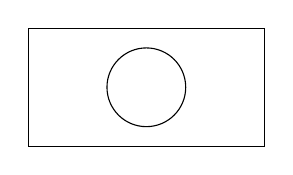
\begin{tikzpicture}
		\draw (0,0) rectangle (3,1.5);
		\draw (1.5,0.75) circle (0.5);
	\end{tikzpicture}
\end{example}

\section{Adding Text Labels}

Use \verb|\node| to place text at a position:

\begin{verbatim}
	\node at (0,0) {Origin};
\end{verbatim}

\begin{center}
	\begin{tikzpicture}
		\draw[->] (0,0) -- (2,0) node[right] {$x$};
		\draw[->] (0,0) -- (0,2) node[above] {$y$};
		\node at (0,0) [below left] {$(0,0)$};
	\end{tikzpicture}
\end{center}

\section{Arrows and Styles}

TikZ provides arrows and line styles:

\begin{itemize}
	\item \verb|->|: Arrow from first to second point
	\item \verb|dashed|, \verb|dotted|: Line styles
	\item \verb|thick|, \verb|ultra thick|: Line weights
\end{itemize}

\begin{example}
	\begin{tikzpicture}
		\draw[->, thick] (0,0) -- (2,1);
		\draw[dashed] (0,0) -- (1,-1);
	\end{tikzpicture}
\end{example}

\section{Simple Tree Structure}

\begin{verbatim}
	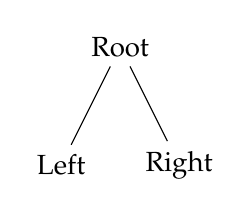
\begin{tikzpicture}
		\node {Root}
		child { node {Left} }
		child { node {Right} };
	\end{tikzpicture}
\end{verbatim}

\begin{center}
	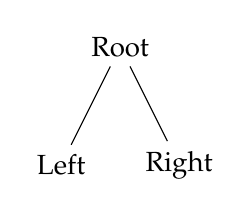
\begin{tikzpicture}
		\node {Root}
		child { node {Left} }
		child { node {Right} };
	\end{tikzpicture}
\end{center}

\section{Coordinate Grid (Optional)}

You can show a grid for layout:

\begin{verbatim}
	\draw[step=1cm, gray, very thin] (0,0) grid (4,4);
\end{verbatim}

\section{Packages for Graphs}

For more advanced graph theory or plots, consider:

\begin{itemize}
	\item \texttt{pgfplots}
	\item \texttt{circuitikz}
	\item \texttt{tkz-graph}
\end{itemize}

\section{Exercise}

\begin{exercise}
	Draw a simple diagram using TikZ:
	\begin{itemize}
		\item A coordinate axis with labels
		\item A rectangle with a circle inside it
		\item A labeled arrow from point $A$ to $B$
		\item A simple binary tree
	\end{itemize}
\end{exercise}

%\chapter{Automation with Makefiles and Scripts}

\section{Why Automate Your Workflow?}

Automation helps when:
\begin{itemize}
	\item You have many `.tex` files to compile
	\item You're using tools like BibTeX, Biber, Glossaries
	\item You want fast, consistent builds without manual steps
\end{itemize}

\section{The Compilation Process}

A typical LaTeX project may require multiple commands:

\begin{itemize}
	\item \texttt{pdflatex main.tex}
	\item \texttt{bibtex main} or \texttt{biber main}
	\item \texttt{makeglossaries main}
	\item \texttt{pdflatex main.tex} (twice)
\end{itemize}

Manually running these every time is inefficient.

\section{Using Makefiles (Unix/Linux/macOS)}

Create a file named `Makefile` (no extension) in your project directory.

\subsection*{Example Makefile}

```makefile
FILE = main

all: pdf

pdf:
pdflatex $(FILE).tex
biber $(FILE)
pdflatex $(FILE).tex
pdflatex $(FILE).tex

clean:
rm -f *.aux *.bbl *.blg *.log *.out *.toc *.lof *.lot
```

\subsection*{Usage}

Open terminal and run:

\begin{verbatim}
	make % builds PDF
	make clean % removes temp files
\end{verbatim}

\section{Cross-Platform Script (Batch for Windows)}

Create a file named \texttt{build.bat}:

\begin{verbatim}
	@echo off
	pdflatex main.tex
	biber main
	pdflatex main.tex
	pdflatex main.tex
	pause
\end{verbatim}

Double-click to run the full build cycle.

\section{Shell Script (Linux/macOS)}

\begin{verbatim}
	#!/bin/bash
	pdflatex main.tex
	biber main
	pdflatex main.tex
	pdflatex main.tex
\end{verbatim}

Make executable:

\begin{verbatim}
	chmod +x build.sh
	./build.sh
\end{verbatim}

\section{Using \texttt{latexmk} (Advanced)}

Install and use \texttt{latexmk}:

\begin{verbatim}
	latexmk -pdf main.tex % Full auto-build
	latexmk -c % Clean temporary files
\end{verbatim}

You can also define a .latexmkrc file for custom rules.

\section{IDE Integration}

Overleaf, TeXstudio, and VS Code (with LaTeX Workshop) support:

\begin{itemize}
	\item Auto-compilation on save
	\item Continuous preview
	\item Custom build sequences
\end{itemize}

\section{Exercise}

\begin{exercise}
	In your LaTeX project directory:
	\begin{itemize}
		\item Create a Makefile or build.bat to compile your project
		\item Add a clean command to delete temporary files
		\item Try using \texttt{latexmk} for automation
	\end{itemize}
\end{exercise}
%\chapter{Best Practices and Troubleshooting}

\section{File Organization}

Organize your project as follows for clarity and scalability:

\begin{verbatim}
	project/
	│
	├── main.tex
	├── chapters/
	│   ├── intro.tex
	│   └── conclusion.tex
	├── figures/
	│   ├── diagram1.pdf
	│   └── chart2.png
	├── bib/
	│   └── references.bib
	└── Makefile
\end{verbatim}

Use \verb|\input{chapters/intro}| or \verb|\include{chapters/conclusion}| to load content modularly.

\section{Use Version Control (Git)}

Track changes and collaborate using Git:

\begin{verbatim}
	git init
	git add .
	git commit -m "Initial LaTeX project"
\end{verbatim}

\textbf{Ignore build files}: Create a `.gitignore` with:

\begin{verbatim}
	*.aux
	*.log
	*.out
	*.toc
	*.bbl
	*.blg
\end{verbatim}

\section{Avoiding Common Errors}

\begin{itemize}
	\item Always match \verb|\begin{...}| with \verb|\end{...}|
	\item Compile twice (or more) for cross-references and TOC
	\item Use `\$...\$` for inline math only — never use double-dollar (`\$\$`) signs
	\item Don’t overload your preamble; only include necessary packages
\end{itemize}

\section{Helpful Debugging Tips}

\begin{itemize}
	\item Look at the first error in the `.log` file — others may cascade
	\item Use Overleaf or an IDE with real-time error highlighting
	\item Comment out blocks to isolate problems quickly
	\item Ensure all images exist and are in the correct format (e.g., PDF, PNG, JPG)
\end{itemize}

\section{Compiler Choices}

\begin{itemize}
	\item \texttt{pdflatex} — best for simple documents
	\item \texttt{xelatex} — supports system fonts and Unicode
	\item \texttt{lualatex} — modern engine with scripting support
\end{itemize}

\section{Package Conflicts}

If your document won’t compile:
\begin{itemize}
	\item Try commenting out recently added packages
	\item Check package versions
	\item Avoid loading the same package multiple times
\end{itemize}

\section{Essential Packages Recap}

\begin{tabular}{ll}
	\texttt{amsmath, amssymb} & Math environments and symbols \\
	\texttt{graphicx} & Include images \\
	\texttt{hyperref} & Clickable references and links \\
	\texttt{biblatex, biber} & Modern bibliography system \\
	\texttt{geometry} & Page layout and margins \\
	\texttt{tikz} & Drawing diagrams
\end{tabular}

\section{Professional Tips}

\begin{itemize}
	\item Use \texttt{\textbackslash autoref} (from \texttt{hyperref}) for context-aware references
	\item Set metadata with \texttt{pdfauthor}, \texttt{pdftitle} via \texttt{hyperref} options
	\item Define your own math macros in the preamble for consistency
\end{itemize}

\section{Exercise}

\begin{exercise}
	Review a LaTeX document you've written and:
	\begin{itemize}
		\item Refactor repeated content into macros
		\item Add version control with Git
		\item Apply a Makefile or automation script
		\item Clean up unused packages and files
	\end{itemize}
\end{exercise}

\end{document}